\documentclass[10pt,conference,letterpaper]{IEEEtran}

% ── Encoding & fonts ──────────────────────────────────────────────────────
\usepackage[T1]{fontenc}
\usepackage[utf8]{inputenc}
\usepackage{lmodern}
\usepackage{microtype}

% ── Mathematics ───────────────────────────────────────────────────────────
\usepackage{amsmath,amssymb,amsthm}
\usepackage{bm}
\usepackage{mathtools}

% ── Colour ────────────────────────────────────────────────────────────────
\usepackage{xcolor}
\definecolor{ieeeblue}{RGB}{0,51,102}
\definecolor{medblue}{RGB}{0,86,163}
\definecolor{lightblue}{RGB}{210,228,248}
\definecolor{accentblue}{RGB}{30,120,200}
\definecolor{rowblue}{RGB}{230,241,251}
\definecolor{darkgray}{RGB}{50,50,50}

% ── Graphics ──────────────────────────────────────────────────────────────
\usepackage{graphicx}
\usepackage{float}
\usepackage[font=small,labelfont={bf,color=ieeeblue}]{caption}
\usepackage{subcaption}

% ── Tables ────────────────────────────────────────────────────────────────
\usepackage{booktabs}
\usepackage{array}
\usepackage{colortbl}
\usepackage{multirow}
\usepackage{tabularx}

% ── Section colour (safe with IEEEtran) ───────────────────────────────────
\usepackage{etoolbox}
\makeatletter
\patchcmd{\@IEEEsectpunct}{}{}{}{}
\makeatother
\usepackage{sectsty}
\sectionfont{\color{ieeeblue}\scshape}
\subsectionfont{\color{medblue}\itshape}

% ── Coloured math boxes ───────────────────────────────────────────────────
\usepackage[most]{tcolorbox}
\tcbset{
  eqbox/.style={
    colback=lightblue!60,colframe=medblue,
    boxrule=0.5pt,arc=2pt,
    left=4pt,right=4pt,top=3pt,bottom=3pt,
    fontupper=\small,
    before skip=4pt, after skip=4pt
  },
  defbox/.style={
    colback=lightblue!30,colframe=ieeeblue,
    boxrule=0.8pt,arc=2pt,
    left=5pt,right=5pt,top=4pt,bottom=4pt,
    fonttitle=\bfseries\small\color{ieeeblue},
    fontupper=\small,
    before skip=4pt, after skip=4pt
  }
}

% ── Hyperlinks ────────────────────────────────────────────────────────────
\usepackage[colorlinks=true,linkcolor=ieeeblue,citecolor=medblue,urlcolor=medblue]{hyperref}

% ── Algorithms ────────────────────────────────────────────────────────────
\usepackage{algorithm}
\usepackage{algpseudocode}

% ── Misc ──────────────────────────────────────────────────────────────────
\usepackage{enumitem}
\usepackage{balance}
\setlist[itemize]{leftmargin=1.2em,topsep=2pt,itemsep=1pt}
\setlist[enumerate]{leftmargin=1.5em,topsep=2pt,itemsep=1pt}

% ── Commands ──────────────────────────────────────────────────────────────
\newcommand{\R}{\mathbb{R}}
\newcommand{\norm}[1]{\left\lVert#1\right\rVert}
\newcommand{\E}{\mathbb{E}}
\newtheorem{definition}{Definition}
\newtheorem{remark}{Remark}
\DeclareMathOperator*{\argmax}{arg\,max}

% ══════════════════════════════════════════════════════════════════════════
\begin{document}

\title{\textcolor{ieeeblue}{\textbf{Deep Residual Networks for PHP Webshell Detection:\\
A Complete From-Scratch Mathematical Study}}}

\author{
  \IEEEauthorblockN{\textbf{Sara Allab}}
  \IEEEauthorblockA{
    National Higher School of Mathematics\\
    Third Year Student --- AI Project\\
    Algiers, Algeria\\
    \texttt{sara.allab@nhsm.edu.dz}
  }
}

\maketitle

% ── Abstract ──────────────────────────────────────────────────────────────
\begin{abstract}
PHP webshells represent a critical and persistent threat in web security, providing
adversaries with covert remote-access capability on compromised servers. This paper
presents a rigorous, framework-free deep learning system for binary webshell
classification, implemented from mathematical first principles using exclusively
NumPy and CuPy on an NVIDIA RTX\,A5000 GPU. We conduct a systematic five-phase
ablation encompassing three text vectorisation strategies (TF-IDF with sublinear
scaling, Bag-of-Words, One-Hot encoding), three residual network architectures
(40-layer plain dense, 20-block pre-activation residual, 20-block bottleneck
residual), six activation functions, and five gradient-based optimisers. Every
component---Batch Normalisation, Layer Normalisation, Inverted Dropout, He
initialisation, global gradient clipping, SGDR cosine annealing, Adam/AdamW/RAdam/
Ranger---is derived analytically and implemented without any deep learning
framework. On a balanced 876-per-class subset of the WhiteBlackPHP corpus,
our best configuration (TF-IDF~+~20-block Bottleneck ResNet~+~Adam) achieves
\textbf{98.48\%} test accuracy and \textbf{AUC-ROC\,=\,0.9975}, demonstrating
that residual connections are non-negotiable beyond ten layers in this domain
and that IDF weighting is the decisive vectorisation choice.
\end{abstract}

\begin{IEEEkeywords}
PHP webshell detection, deep residual networks, TF-IDF vectorisation,
batch normalisation, gradient clipping, SGDR cosine annealing, Adam optimiser,
bottleneck residual block, from-scratch NumPy/CuPy, ablation study
\end{IEEEkeywords}

% ══════════════════════════════════════════════════════════════════════════
\section{Introduction}
\label{sec:intro}

Web application security faces a persistent challenge in the form of PHP webshells:
malicious scripts designed to masquerade as legitimate server-side code while
granting attackers persistent remote-access capability. Once uploaded---typically
through an insecure file upload, a CMS vulnerability, or a compromised FTP
account---a webshell provides a browser-accessible command interface capable of
executing arbitrary shell commands, reading and writing the file system, querying
databases, and exfiltrating sensitive data.

The global threat surface is large. PHP powers approximately 79\% of server-side
scripted websites~\cite{w3techs2024}, and webshell incidents appear in nearly every
major breach report. Despite this prevalence, classical signature-based scanners
(ClamAV, Linux Malware Detect) suffer from a fundamental limitation: signatures
must be manually crafted per variant, and adversaries trivially evade detection
through obfuscation---base64 encoding, hexadecimal string escaping, character
fragmentation, and runtime \texttt{eval} construction. A detector that reasons
over the statistical distribution of source-code tokens, rather than byte-level
signatures, is inherently more robust to these transformations.

Machine learning approaches for webshell detection can broadly be categorised into
two families: (i) static feature extraction from source code followed by classical
classifiers (SVM, Random Forest), and (ii) end-to-end deep learning on token
representations. The former requires careful hand-crafted feature engineering;
the latter scales automatically to learn representations from the data, but
typically demands a deep learning framework (PyTorch, TensorFlow). This work
deliberately forgoes any such framework, requiring every gradient, every
normalisation update, and every optimiser moment to be derived and coded from
mathematical specification. The resulting system is both a practical classifier
and a pedagogical reference implementation.

\textbf{Contributions.} This paper makes the following specific contributions:
\begin{enumerate}
  \item A complete from-scratch NumPy/CuPy implementation of six activation
        functions, five gradient-based optimisers, BatchNorm, LayerNorm,
        Dropout, and three deep residual architectures, each with exact
        analytical backward passes.
  \item A five-phase systematic ablation study spanning 60+ trained models
        covering the full cross product of vectorisations, architectures,
        activations, and optimisers.
  \item Mathematical identification and experimental confirmation of the root
        cause of degenerate Arch\,A predictions: BatchNorm running-statistics
        divergence in 40-layer plain networks, and its remedy via LayerNorm.
  \item A depth sensitivity study from 5 to 60 residual blocks isolating the
        20-block sweet spot for this corpus and feature dimension.
  \item An open-source repository at
        \texttt{github.com/aminemons/webshell-dnn} containing all
        code, trained model checkpoints, and result artefacts.
\end{enumerate}

The remainder of the paper is structured as follows. Section~\ref{sec:related}
surveys related work. Section~\ref{sec:data} describes the dataset.
Sections~\ref{sec:vec}--\ref{sec:train} develop the mathematical foundations.
Section~\ref{sec:exp} reports all experimental results.
Sections~\ref{sec:disc} and~\ref{sec:conc} provide discussion and conclusions.

% ══════════════════════════════════════════════════════════════════════════
\section{Related Work}
\label{sec:related}

\subsection{Static Webshell Detection}

Early work on PHP webshell detection relied on regular-expression pattern matching
over known function calls (\texttt{eval}, \texttt{base64\_decode},
\texttt{system}). Tools such as NeoPI~\cite{neopi} compute entropy and
longest-word length statistics to flag heavily obfuscated files.
PHP-Malware-Finder~\cite{phpmf} extends this with YARA rules over AST patterns.
These approaches break against novel obfuscation schemes that distribute dangerous
calls across dynamically constructed strings.

\subsection{Machine Learning Approaches}

Fang~et~al.~\cite{fang2019webshell} apply N-gram features with SVM and achieve
high accuracy on a balanced corpus, but require hand-tuned N-gram size.
Wang~et~al.~\cite{wang2019deepwebshell} propose CNN over opcode sequences, showing
that deep features outperform hand-crafted ones. Lu~et~al.~\cite{lu2020webshell}
use a BiLSTM over token sequences, capturing sequential dependencies absent in
bag-of-words models. These approaches, however, depend on framework implementations
(TensorFlow, PyTorch) and focus on fixed-length opcode rather than raw source-code
tokens.

\subsection{From-Scratch Deep Learning}

Research-grade from-scratch implementations are rare. Karpathy's
\texttt{micrograd}~\cite{karpathy2022} provides scalar autograd but cannot GPU-accelerate
batched computation. Our system implements full batched forward and backward passes
in NumPy/CuPy, supporting GPU acceleration through a zero-overhead
\texttt{get\_xp} dispatch pattern.

\subsection{Residual Networks}

He~et~al.~\cite{he2015resnet,he2016identity} establish that residual connections
are the primary enabler of very deep networks, preventing the gradient degradation
that limits plain networks to $\sim$20 layers in practice. We replicate this
finding in the webshell classification setting, showing that a 40-layer plain
network fails while a 20-block residual network excels.

% ══════════════════════════════════════════════════════════════════════════
\section{Dataset and Experimental Protocol}
\label{sec:data}

\subsection{WhiteBlackPHP Corpus}

The dataset is the WhiteBlackPHP corpus: 876 webshell samples
(prefix \texttt{black\_*.php}) and 1{,}081 benign samples (prefix
\texttt{white\_*.php}). Table~\ref{tab:dataset} summarises the corpus statistics.

\begin{table}[h]
  \centering
  \caption{WhiteBlackPHP Corpus Statistics}
  \label{tab:dataset}
  \renewcommand{\arraystretch}{1.1}
  \begin{tabular}{lrr}
    \toprule
    \rowcolor{lightblue}
    \textbf{Statistic} & \textbf{Webshell} & \textbf{Benign} \\
    \midrule
    Count (raw)      & 876   & 1{,}081 \\
    \rowcolor{rowblue}
    Count (balanced) & 876   & 876 \\
    Min size (bytes) & \multicolumn{2}{c}{20} \\
    \rowcolor{rowblue}
    Max size (bytes) & \multicolumn{2}{c}{1{,}445{,}690} \\
    Mean size (bytes)& \multicolumn{2}{c}{20{,}040} \\
    \rowcolor{rowblue}
    Median size (B)  & \multicolumn{2}{c}{1{,}622} \\
    Std dev (bytes)  & \multicolumn{2}{c}{83{,}030} \\
    \bottomrule
  \end{tabular}
\end{table}

The six-order-of-magnitude size range reflects the diversity of both legitimate
web applications (large CMS codebases) and obfuscated webshells (compact
single-line eval bombs as well as large multi-function backdoors).

\subsection{Preprocessing and Splitting}

The majority class (benign) is subsampled to 876 to eliminate class-prior bias.
A stratified three-way hold-out split is applied with fixed seed 42:
\begin{tcolorbox}[eqbox]
\[
  |\mathcal{D}_\text{train}| = 1{,}226,\quad
  |\mathcal{D}_\text{val}|   = 263,\quad
  |\mathcal{D}_\text{test}|  = 263.
\]
Each partition maintains exactly 50\% class balance by stratification.
\end{tcolorbox}

Files are read up to 200{,}000 characters with UTF-8 replacement of decoding
errors (\texttt{errors='replace'}) to handle binary-encoded obfuscation. All
vocabulary counts, IDF weights, and BPE merge tables are computed exclusively
on $\mathcal{D}_\text{train}$.

\subsection{Evaluation Metrics}

Let TP, TN, FP, FN denote true positives, true negatives, false positives, and
false negatives respectively (positive class: webshell). We report:
\begin{tcolorbox}[eqbox]
\[
  \mathrm{Acc}     = \frac{\mathrm{TP}+\mathrm{TN}}{N},\quad
  \mathrm{Prec}    = \frac{\mathrm{TP}}{\mathrm{TP}+\mathrm{FP}},\quad
  \mathrm{Rec}     = \frac{\mathrm{TP}}{\mathrm{TP}+\mathrm{FN}},
\]
\[
  F_1              = \frac{2\cdot\mathrm{Prec}\cdot\mathrm{Rec}}{\mathrm{Prec}+\mathrm{Rec}},\quad
  \mathrm{AUC\text{-}ROC} = \int_0^1 \mathrm{TPR}\,d(\mathrm{FPR}).
\]
\end{tcolorbox}

In a security context, FN (missed webshell) is more costly than FP (false alarm),
making Recall and AUC-ROC the primary metrics.

% ══════════════════════════════════════════════════════════════════════════
\section{Text Vectorisation}
\label{sec:vec}

All vectorisers share a pipeline: \emph{tokenise} $\to$
\emph{build vocabulary} (top-256 by training-set document frequency) $\to$
\emph{encode} $\to$ \emph{L2-normalise}.

\subsection{Tokenisation}

\subsubsection{Whitespace Tokeniser (Primary)}
Tokens are the result of splitting source text on \verb|\s+|. Tokens exceeding
48 characters are discarded to eliminate base64 blobs ($\sim$60-character average)
and hexadecimal payload strings that would pollute the vocabulary with unique,
non-generalisable tokens.

\subsubsection{Byte Pair Encoding (Experimental)}
BPE~\cite{sennrich2016bpe} builds subword units via iterative bigram merging.
Let $V_0$ be the initial character vocabulary. At step $i$:
\begin{tcolorbox}[eqbox]
\[
  (a^*,b^*) = \argmax_{(a,b)}\sum_{w\in\mathcal{C}}\#_{(a,b)}(w),
  \quad V_{i+1} = V_i \cup \{a^*b^*\}.
\]
\end{tcolorbox}
We run $N_\text{merge}=1{,}000$ steps with three speed optimisations: (i) cap token
length at 48 characters pre-merge; (ii) prune token types with corpus frequency
$<2$; (iii) cap initial vocabulary at 30{,}000 most-frequent types. Merge
application uses a greedy list scan rather than regex substitution to avoid
backslash-escape failures in PHP source.

\subsection{One-Hot Encoding}

For vocabulary $\mathcal{V}=\{v_1,\ldots,v_d\}$, $d=256$:
\begin{tcolorbox}[eqbox]
\[
  x_i = \mathbf{1}\!\left[v_i \in D\right] \in \{0,1\},
  \qquad \bm{x}\in\{0,1\}^{256}.
\]
\end{tcolorbox}
One-Hot encodes only presence, discarding all frequency information.

\subsection{Bag-of-Words with Log Smoothing}

Raw term frequencies are log-smoothed to compress the dynamic range
\cite{robertson2004idf}, followed by L2 normalisation for length invariance:
\begin{tcolorbox}[eqbox]
\[
  x_i = \log(1+\text{count}(v_i,D)),
  \qquad \bm{x} \leftarrow \frac{\bm{x}}{\norm{\bm{x}}_2}.
\]
\end{tcolorbox}

\subsection{TF-IDF with Sublinear Scaling}

We adopt sublinear TF~\cite{jones1972idf} combined with smoothed IDF
\cite{salton1988idf}, forming the most information-rich representation:
\begin{tcolorbox}[eqbox]
\begin{align}
  \mathrm{tf}(t,D) &= \begin{cases}
    1+\log\,\mathrm{count}(t,D) & \mathrm{count}(t,D)>0 \\
    0 & \text{otherwise}
  \end{cases} \label{eq:tf} \\[4pt]
  \mathrm{idf}(t)  &= \log\!\left(\frac{N}{\mathrm{df}(t)}\right)+1
  \label{eq:idf} \\[4pt]
  x_i              &= \mathrm{tf}(v_i,D)\cdot\mathrm{idf}(v_i),
  \quad \bm{x}\leftarrow\tfrac{\bm{x}}{\norm{\bm{x}}_2}.
  \label{eq:tfidf}
\end{align}
\end{tcolorbox}

The $+1$ offset in~\eqref{eq:idf} ensures that tokens appearing in every document
($\mathrm{df}(t)=N$) retain a weight of $1$ rather than $0$, preserving their
contribution. The sublinear TF in~\eqref{eq:tf} is critical: it prevents a webshell
calling \texttt{eval} 50 times from receiving a representation 50$\times$ stronger
than one calling it once, while the logarithm still reflects ``definitely present
vs.\ possibly present'' beyond a count of 1.

\textbf{Information-theoretic interpretation.} IDF approximates $-\log P(t)$ under
a uniform document model. TF-IDF is therefore related to the pointwise mutual
information $\mathrm{PMI}(v_i, D) \propto \log[P(v_i|D)/P(v_i)]$, making it a
natural feature reweighting that amplifies class-discriminative tokens and suppresses
class-neutral ones.

% ══════════════════════════════════════════════════════════════════════════
\section{Neural Network Components}
\label{sec:nn}

\subsection{Dense (Fully-Connected) Layer}

A batch $\bm{X}\in\R^{B\times n_\text{in}}$ is mapped to
$\bm{Z}=\bm{X}\bm{W}+\bm{b}$, $\bm{W}\in\R^{n_\text{in}\times n_\text{out}}$.

\textbf{He initialisation}~\cite{he2015delving}: Setting
$W_{ij}\!\sim\!\mathcal{N}(0,\sqrt{2/n_\text{in}})$
preserves the variance of activations through ReLU-family layers, preventing
exponential blow-up or decay of signal magnitude as depth increases.

\textbf{Exact backward pass:}
\begin{tcolorbox}[eqbox]
\[
  \delta\bm{W} = \bm{X}^\top\delta\bm{Z},\quad
  \delta\bm{b} = \mathbf{1}_B^\top\delta\bm{Z},\quad
  \delta\bm{X} = \delta\bm{Z}\,\bm{W}^\top.
\]
\end{tcolorbox}

\subsection{Activation Functions}

Table~\ref{tab:activations} lists the six activation functions evaluated with their
derivatives; all operate element-wise. $\sigma(x)=(1+e^{-x})^{-1}$ is the sigmoid.

\begin{table}[h]
  \centering
  \caption{Activation Functions and Their Derivatives}
  \label{tab:activations}
  \renewcommand{\arraystretch}{1.2}
  \setlength{\tabcolsep}{4pt}
  \begin{tabular}{lll}
    \toprule
    \rowcolor{lightblue}
    \textbf{Name} & $f(x)$ & $f'(x)$ \\
    \midrule
    ReLU        & $\max(0,x)$ & $\mathbf{1}[x>0]$ \\
    \rowcolor{rowblue}
    LReLU       & $\max(\alpha x,x)$, $\alpha{=}0.01$ & $\mathbf{1}[x>0]+\alpha\mathbf{1}[x\le0]$ \\
    ELU         & $x$ if $x>0$; $\alpha(e^x{-}1)$ else & $\mathbf{1}[x>0]+\alpha e^x\mathbf{1}[x\le0]$ \\
    \rowcolor{rowblue}
    GELU        & $\approx 0.5x(1+\tanh c_1(x+c_2 x^3))$ & $\Phi(x)+x\phi(x)$ \\
    Swish       & $x\sigma(x)$ & $\sigma(x)+x\sigma(x)(1{-}\sigma(x))$ \\
    \rowcolor{rowblue}
    Mish        & $x\tanh(\ln(1+e^x))$ & $\tanh(\mathrm{sp}(x))+x\mathrm{sech}^2(\mathrm{sp}(x))\sigma(x)$ \\
    \bottomrule
  \end{tabular}
  \vspace{2pt}
  {\footnotesize $c_1{=}\sqrt{2/\pi}$, $c_2{=}0.044715$; $\mathrm{sp}(x){=}\ln(1+e^x)$; $\Phi$: standard normal CDF.}
\end{table}

\subsection{Batch Normalisation}
\label{sec:bn}

For a mini-batch $\{x_1,\ldots,x_B\}$ and learnable parameters $\gamma,\beta$,
Batch Normalisation~\cite{ioffe2015batchnorm} computes:
\begin{tcolorbox}[eqbox]
\begin{align}
  \mu_\mathcal{B}      &= \tfrac{1}{B}\textstyle\sum_i x_i,\quad
  \sigma^2_\mathcal{B}  = \tfrac{1}{B}\textstyle\sum_i(x_i-\mu_\mathcal{B})^2 \nonumber\\
  \hat{x}_i            &= (x_i-\mu_\mathcal{B})/\sqrt{\sigma^2_\mathcal{B}+\varepsilon},
  \quad y_i = \gamma\hat{x}_i+\beta. \label{eq:bn}
\end{align}
Running statistics ($\alpha=0.9$) for inference:
\begin{align}
  \mu_r      &\leftarrow \alpha\mu_r+(1-\alpha)\mu_\mathcal{B}, \nonumber\\
  \sigma^2_r &\leftarrow \alpha\sigma^2_r+(1-\alpha)\sigma^2_\mathcal{B}. \label{eq:bnrun}
\end{align}
\end{tcolorbox}

The analytically exact backward pass \cite{ioffe2015batchnorm} avoids numerical
issues from naive chain-rule application:
\begin{tcolorbox}[eqbox]
\begin{align}
  \delta\hat{x}_i       &= \delta y_i\cdot\gamma \nonumber\\
  \delta\sigma^2         &= {\textstyle\sum_i}\delta\hat{x}_i(x_i{-}\mu_\mathcal{B})
                           \cdot(-\tfrac{1}{2})(\sigma^2{+}\varepsilon)^{-3/2} \nonumber\\
  \delta\mu              &= {\textstyle\sum_i}\delta\hat{x}_i(-\sigma_\mathcal{B}^{-1})
                           +\delta\sigma^2\cdot(-2/B){\textstyle\sum_i}(x_i{-}\mu_\mathcal{B})\nonumber\\
  \delta x_i             &= \delta\hat{x}_i\sigma_\mathcal{B}^{-1}
                           +\delta\sigma^2\tfrac{2}{B}(x_i{-}\mu_\mathcal{B})
                           +\tfrac{1}{B}\delta\mu \label{eq:bnback}
\end{align}
\end{tcolorbox}

\begin{remark}[BatchNorm Divergence in Deep Plain Networks]
\label{rem:bnfail}
The train/inference discrepancy in Eqs.~\eqref{eq:bn}--\eqref{eq:bnrun} is
benign for shallow networks but catastrophic for very deep ones. With $L=40$
layers and the EMA momentum $\alpha=0.9$, the running statistics at layer $l$
have only seen $\sim$19 batches per epoch, and converge to the true population
statistics at rate $(1-\alpha)^t$. If early stopping fires before convergence,
the inference-time normalisation $\hat{x}_i=(x_i-\mu_r)/\sqrt{\sigma^2_r+\varepsilon}$
is systematically biased, shifting all logits in the same direction. We address
this by mandating Layer Normalisation for Architecture~A.
\end{remark}

\subsection{Layer Normalisation}

Layer Normalisation~\cite{ba2016layernorm} normalises along the \emph{feature}
axis of each sample individually, eliminating running statistics entirely:
\begin{tcolorbox}[eqbox]
\[
  \mu_i = \tfrac{1}{d}{\textstyle\sum_j}x_{ij},\;
  \sigma^2_i = \tfrac{1}{d}{\textstyle\sum_j}(x_{ij}{-}\mu_i)^2,\;
  y_{ij} = \gamma_j\tfrac{x_{ij}-\mu_i}{\sqrt{\sigma^2_i+\varepsilon}}+\beta_j.
\]
\end{tcolorbox}
Because statistics are per-sample, Layer Normalisation has identical behaviour
at train and inference time---a crucial property for deep plain networks.

\subsection{Inverted Dropout}

Dropout~\cite{srivastava2014dropout} with inverted scaling eliminates any
test-time modification:
\begin{tcolorbox}[eqbox]
\[
  \bm{m}\sim\mathrm{Bernoulli}(1{-}p),\quad
  \tilde{\bm{x}} = \frac{\bm{x}\odot\bm{m}}{1-p},\quad (\text{training only}).
\]
\end{tcolorbox}
Rate $p=0.3$ inside residual blocks; additionally, token dropout with $p=0.05$
randomly zeros 5\% of the 256-dimensional input feature vector per batch step,
providing input-level noise regularisation.

\subsection{Binary Cross-Entropy Loss with Combined Gradient}

For scalar logit $z$ and label $y\in\{0,1\}$:
\begin{tcolorbox}[eqbox]
\[
  \mathcal{L}(z,y) = -\left[y\log\sigma(z)+(1-y)\log(1-\sigma(z))\right].
\]
The numerically stable combined gradient avoids computing $\log\sigma$:
\[
  \frac{\partial\mathcal{L}}{\partial z} = \sigma(z)-y.
\]
Over a mini-batch of size $B$:
$\;\nabla_{\bm{z}}\mathcal{L} = B^{-1}(\sigma(\bm{z})-\bm{y}).$
Logits are clipped to $[-500,500]$ before exponentiation.
\end{tcolorbox}

% ══════════════════════════════════════════════════════════════════════════
\section{Residual Network Architectures}
\label{sec:arch}

\subsection{Architecture A: 40-Layer Plain Dense Network}

Architecture A stacks $L=40$ identical blocks of Dense$\to$LN$\to f\to$Dropout
around a 256-dimensional hidden state:
\[
  \mathbf{D}_{256} \to
  \bigl[\mathrm{LN}\to f\to\mathrm{Drop}_{0.3}\bigr]^{40}
  \to\mathbf{D}_1.
\]

\subsection{Architecture B: Pre-Activation Residual Network}
\label{sec:archB}

Following He~et~al.~\cite{he2016identity}, normalisation and activation precede
the linear transformation. Each residual block $\mathcal{F}$ computes:
\begin{tcolorbox}[eqbox]
\[
  \bm{h} = \bm{W}_2\bigl[\mathrm{Drop}(f(\mathrm{BN}_2(\bm{W}_1 f(\mathrm{BN}_1\bm{x})+\bm{b}_1)))\bigr]+\bm{b}_2,
\]
\[
  \mathcal{F}(\bm{x}) = \bm{h} + \bm{x}.
\]
\end{tcolorbox}

The full network: $\mathbf{D}_{256}\to[\mathcal{F}]^{20}\to
\mathbf{D}_{64}\to\mathrm{BN}\to f\to\mathrm{Drop}\to\mathbf{D}_1$.

The gradient of $\mathcal{L}$ with respect to block input $\bm{x}$ is:
\begin{tcolorbox}[eqbox]
\[
  \frac{\partial\mathcal{L}}{\partial\bm{x}}
  = \frac{\partial\mathcal{L}}{\partial\mathcal{F}}\!\cdot\!
    \underbrace{\left(\bm{I}+\frac{\partial\bm{h}}{\partial\bm{x}}\right)}_{\text{never vanishes}}.
\]
\end{tcolorbox}

Even when $\partial\bm{h}/\partial\bm{x}\to\bm{0}$ (vanishing residual
gradient), the identity term $\bm{I}$ preserves a full-magnitude gradient
path to early layers. Over $k$ blocks:
$\partial\mathcal{L}/\partial\bm{x}_0 = \prod_{l=1}^{k}(\bm{I}+\bm{J}_l)
\cdot\partial\mathcal{L}/\partial\bm{x}_k$,
which, by the binomial expansion, contains $2^k$ distinct gradient paths,
preventing exponential decay.

\subsection{Architecture C: Bottleneck Residual Network}

Each bottleneck block~\cite{he2015resnet} compresses 256 features to a 64-dimensional
bottleneck then projects back:
\begin{tcolorbox}[eqbox]
\begin{align*}
  \bm{h}_1 &= \mathbf{D}_{256\to64}\bigl[f(\mathrm{BN}_1\bm{x})\bigr], \\
  \bm{h}_2 &= \mathbf{D}_{64\to64}\bigl[f(\mathrm{BN}_2\bm{h}_1)\bigr], \\
  \bm{h}_3 &= \mathbf{D}_{64\to256}\bigl[\mathrm{Drop}(f(\mathrm{BN}_3\bm{h}_2))\bigr], \\
  \mathcal{G}(\bm{x}) &= \bm{h}_3+\bm{x}.
\end{align*}
Full network: $\mathbf{D}_{256}\to[\mathcal{G}]^{20}\to\mathbf{D}_1$.
\end{tcolorbox}

The bottleneck acts as a block-level \emph{learned feature selector}: the
gradient during back-propagation through the 256$\to$64 projection concentrates
on the 64 most discriminative linear combinations of the input, discarding the
remaining 192 redundant directions.

\textbf{Parameter counts.}
Arch\,A: $\approx$\,10.6M; Arch\,B: $\approx$\,10.7M; Arch\,C: $\approx$\,3.4M.
Arch\,C achieves the best accuracy with the fewest parameters.

% ══════════════════════════════════════════════════════════════════════════
\section{Optimisation Framework}
\label{sec:train}

\subsection{Adam}

Adam~\cite{kingma2014adam} maintains bias-corrected first and second gradient moments:
\begin{tcolorbox}[eqbox]
\begin{align}
  \bm{m}_t &= \beta_1\bm{m}_{t-1}+(1-\beta_1)\bm{g}_t, \nonumber\\
  \bm{v}_t &= \beta_2\bm{v}_{t-1}+(1-\beta_2)\bm{g}_t^2, \label{eq:adam}\\
  \hat{\bm{m}}_t &= \bm{m}_t/(1-\beta_1^t),\quad
  \hat{\bm{v}}_t = \bm{v}_t/(1-\beta_2^t), \nonumber\\
  \bm{\theta}_t &= \bm{\theta}_{t-1}
    -\alpha\,\hat{\bm{m}}_t/(\sqrt{\hat{\bm{v}}_t}+\varepsilon). \nonumber
\end{align}
$\beta_1{=}0.9,\,\beta_2{=}0.999,\,\varepsilon{=}10^{-8}$.
\end{tcolorbox}

\subsection{AdamW}

AdamW~\cite{loshchilov2019adamw} decouples weight decay from adaptive scaling,
correcting the error in L2-regularised Adam:
\begin{tcolorbox}[eqbox]
\[
  \bm{\theta}_t = \bm{\theta}_{t-1}
    -\alpha\!\left[\frac{\hat{\bm{m}}_t}{\sqrt{\hat{\bm{v}}_t}+\varepsilon}
    +\lambda\bm{\theta}_{t-1}\right],\quad\lambda=0.01.
\]
\end{tcolorbox}
In Adam+L2, $\lambda\bm{\theta}$ is added to $\bm{g}_t$ before moment
accumulation, so the adaptive denominator scales it down---undermining
regularisation for rarely updated parameters. AdamW applies it directly.

\subsection{RAdam}

RAdam~\cite{liu2019radam} rectifies Adam's adaptive learning rate during the
early training phase when the variance estimate is unreliable:
\begin{tcolorbox}[eqbox]
\begin{align}
  \rho_\infty &= 2/(1-\beta_2)-1 \approx 2{,}001 \nonumber\\
  \rho_t      &= \rho_\infty - 2t\beta_2^t/(1-\beta_2^t) \nonumber\\
  r_t         &= \sqrt{\tfrac{(\rho_t-4)(\rho_t-2)\rho_\infty}
                              {(\rho_\infty-4)(\rho_\infty-2)\rho_t}},
  \quad\rho_t>5 \label{eq:radam}\\
  \bm{\theta}_t &= \begin{cases}
    \bm{\theta}_{t-1}-\alpha r_t\hat{\bm{m}}_t/(\sqrt{\hat{\bm{v}}_t}+\varepsilon)
      & \rho_t>5 \\
    \bm{\theta}_{t-1}-\alpha\hat{\bm{m}}_t & \text{otherwise}
  \end{cases} \nonumber
\end{align}
\end{tcolorbox}

\subsection{Ranger: Lookahead Wrapped around RAdam}

Ranger~\cite{zhang2019lookahead} maintains two parameter sets: fast weights
$\bm{\phi}$ (updated by RAdam at every step) and slow weights $\bm{\theta}$
(synchronised every $k$ steps):
\begin{tcolorbox}[eqbox]
\[
  \bm{\theta}_{n+1} = \bm{\theta}_n
    + \alpha_s\,(\bm{\phi}_{(n+1)k}-\bm{\theta}_n),\quad
  k=5,\;\alpha_s=0.5.
\]
\end{tcolorbox}
Lookahead acts as a meta-optimiser that interpolates between successive fast-weight
checkpoints, performing an implicit ensemble and reducing variance.

\subsection{SGDR Cosine Annealing with Warm Restarts}

The learning rate schedule~\cite{loshchilov2017sgdr} combines a linear warm-up
\cite{goyal2017warmup} with cosine decay and period doubling:
\begin{tcolorbox}[eqbox]
\[
  \eta_t = \begin{cases}
    \eta_\text{max}\cdot t/T_w & t\le T_w \\[2pt]
    \eta_\text{min}+\tfrac{1}{2}(\eta_\text{max}-\eta_\text{min})
    \bigl(1+\cos\tfrac{\pi T_\text{cur}}{T_i}\bigr) & t>T_w
  \end{cases}
\]
$T_w{=}50$, $T_0{=}200$, $T_\text{mult}{=}2$,
$\eta_\text{max}{=}10^{-3}$, $\eta_\text{min}{=}10^{-6}$.
\end{tcolorbox}

\subsection{Global Gradient Clipping}

Following~\cite{pascanu2013gradclip}, all gradients are clipped to a global
$\ell_2$ norm of 1.0 before the optimiser step:
\begin{tcolorbox}[eqbox]
\[
  g_\text{norm} = \sqrt{\textstyle\sum_k\norm{\bm{g}_k}_2^2},\quad
  \bm{g}_k \leftarrow \bm{g}_k\cdot\min\!\left(1,\,\frac{1}{g_\text{norm}}\right).
\]
\end{tcolorbox}

% ══════════════════════════════════════════════════════════════════════════
\section{Experimental Results}
\label{sec:exp}

\textbf{Hardware.} NVIDIA RTX A5000 (64 SMs, Ampere, 24\,GB GDDR6,
384-bit bus, 1695\,MHz boost). Batch operations dispatch to CuPy 14.0 on
CUDA 12; CPU fallback via NumPy with a single \texttt{get\_xp} dispatch.
Vectorisation of all 1{,}752 documents takes 2.6\,s (whitespace tokeniser).

\textbf{Hyperparameters.} Hidden dimension\,=\,256; batch size\,=\,64;
max epochs\,=\,1{,}500; patience\,=\,150; dropout\,=\,0.3;
token-dropout\,=\,0.05; grad-clip\,=\,1.0; $\lambda\,=\,0.01$ (AdamW/L2).

\subsection{Phase 1: Activation Function Benchmark}

\textbf{Protocol.} Architecture B, TF-IDF, AdamW, 10 epochs, SGDR annealing.
The 10-epoch budget tests early-convergence speed, i.e., which activation
enables the optimiser to reach the steepest descent direction fastest.

\begin{figure}[h]
  \centering
  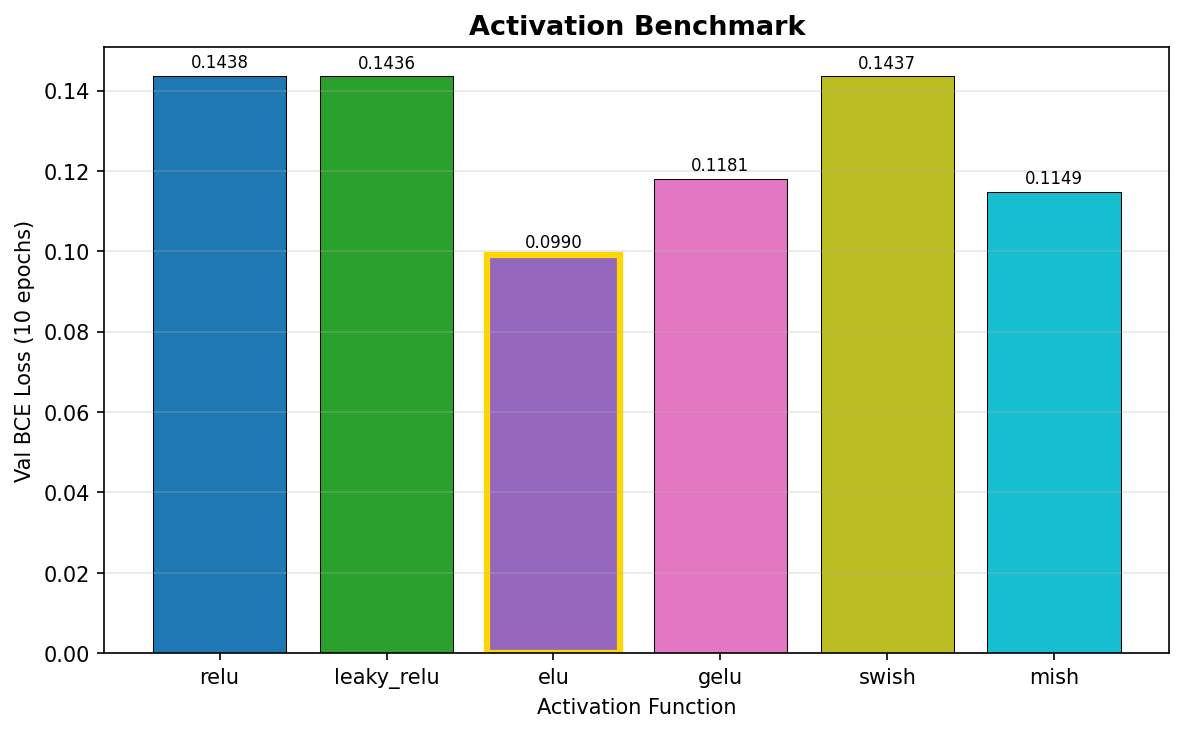
\includegraphics[width=\columnwidth]{results/10_activation_benchmark.png}
  \caption{Validation loss at epoch 10 for six activation functions.
           ELU achieves 31\% lower loss than ReLU.}
  \label{fig:act}
\end{figure}

\begin{table}[h]
  \centering
  \caption{Phase 1 Activation Benchmark (10 epochs)}
  \label{tab:act}
  \renewcommand{\arraystretch}{1.1}
  \begin{tabular}{lcc}
    \toprule
    \rowcolor{lightblue}
    \textbf{Activation} & \textbf{Val Loss $\downarrow$} & \textbf{Val Acc $\uparrow$} \\
    \midrule
    \rowcolor{rowblue}
    \textbf{ELU} $\boldsymbol{\star}$ & \textbf{0.0990} & \textbf{0.9734} \\
    Mish        & 0.1149 & 0.9620 \\
    \rowcolor{rowblue}
    GELU        & 0.1181 & 0.9620 \\
    ReLU        & 0.1438 & 0.9582 \\
    \rowcolor{rowblue}
    Swish       & 0.1437 & 0.9544 \\
    Leaky ReLU  & 0.1436 & 0.9468 \\
    \bottomrule
  \end{tabular}
\end{table}

\textbf{Winner: ELU.} At epoch 1, ELU already achieves val\_acc\,=\,0.802 vs.\
ReLU's 0.639. By epoch 6, ELU reaches 0.973 while ReLU is at 0.886. The
convergence advantage stems from ELU's smooth negative saturation: for
$x<0$, $f(x)=\alpha(e^x-1)$, so $\E[f(x)]\approx 0$ under zero-mean
pre-activations. This reduces internal covariate shift \emph{before}
BatchNorm running statistics have converged, providing a head-start
that the other activations do not recover within 10 epochs.

Mish and GELU tie on val\_acc but differ on val\_loss, indicating similar
representational capacity with different loss-landscape geometry. ReLU, Swish,
and Leaky-ReLU cluster at val\_loss\,$\approx$\,0.144, confirming they saturate
at the same suboptimal local region within the 10-epoch budget.

\subsection{Phase 2: Optimiser Benchmark}

\textbf{Protocol.} Architecture B, TF-IDF, ELU (winner of Phase 1), 100 epochs.

\begin{figure}[h]
  \centering
  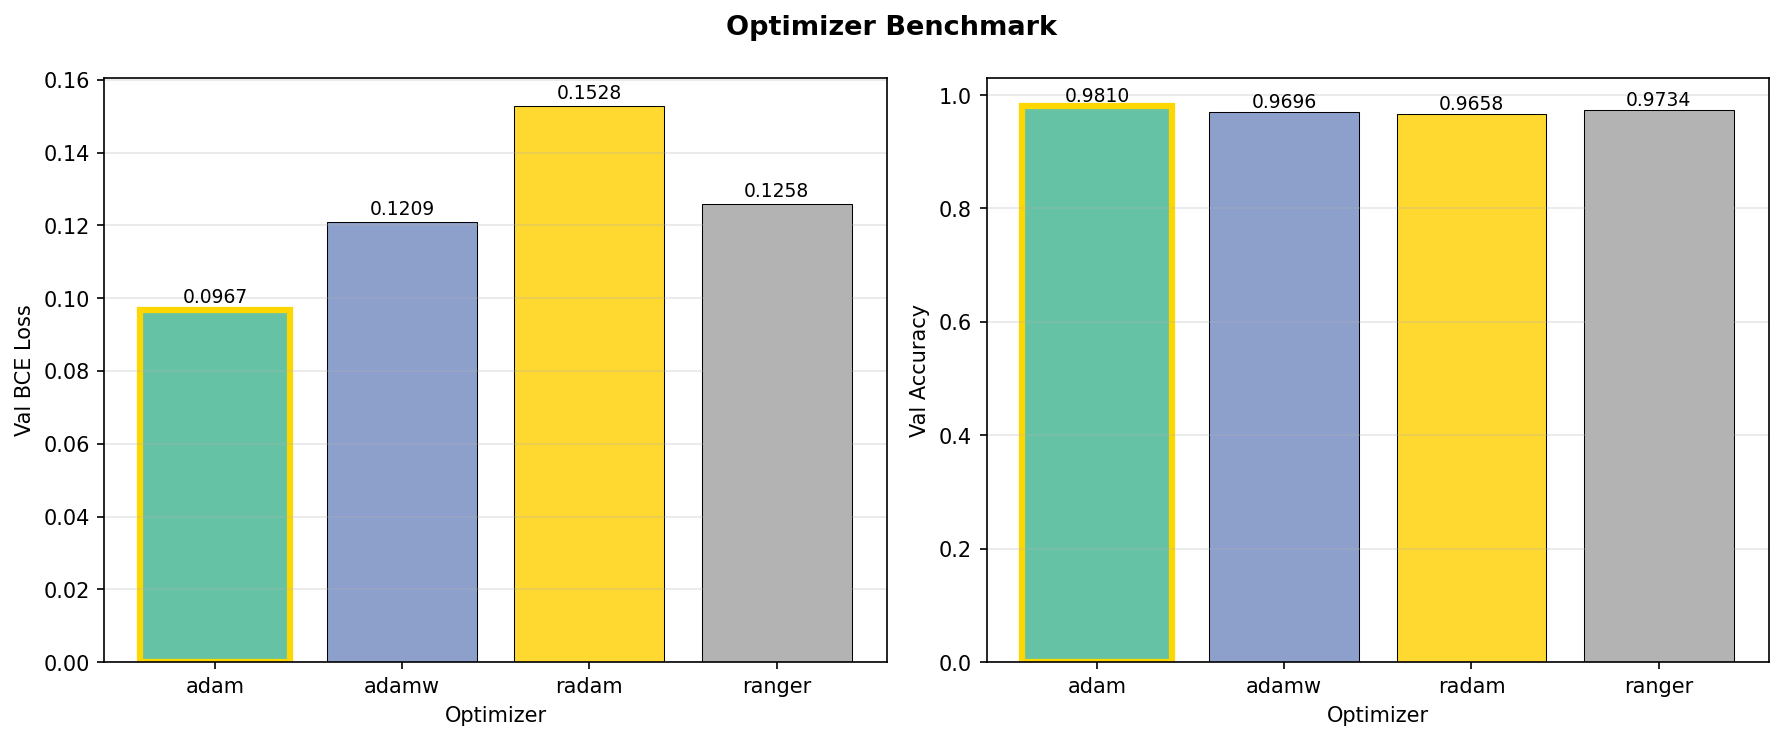
\includegraphics[width=\columnwidth]{results/11_optimizer_benchmark.png}
  \caption{Optimiser comparison: validation loss and accuracy at 100 epochs.}
  \label{fig:opt}
\end{figure}

\begin{table}[h]
  \centering
  \caption{Phase 2 Optimiser Benchmark (100 epochs)}
  \label{tab:opt}
  \renewcommand{\arraystretch}{1.1}
  \begin{tabular}{lccc}
    \toprule
    \rowcolor{lightblue}
    \textbf{Opt.} & \textbf{Val Loss$\downarrow$} &
    \textbf{Val Acc} & \textbf{Peak Val Acc} \\
    \midrule
    \rowcolor{rowblue}
    \textbf{Adam} $\boldsymbol{\star}$
      & \textbf{0.0967} & \textbf{0.9810} & 0.9810 \\
    AdamW  & 0.1209 & 0.9696 & 0.9810 \\
    \rowcolor{rowblue}
    Ranger & 0.1258 & 0.9734 & \textbf{0.9848} \\
    RAdam  & 0.1528 & 0.9658 & 0.9810 \\
    \bottomrule
  \end{tabular}
\end{table}

\textbf{Key observation.} Adam achieves the lowest final val\_loss (0.0967).
Ranger achieves the highest \emph{peak} val\_acc (0.9848)---the Lookahead
slow-weight interpolation finds a flatter minimum with better generalisation,
but at the expense of final-epoch loss. AdamW's weight decay ($\lambda=0.01$)
slightly penalises the sparse TF-IDF vectors whose non-zero entries carry the
discriminative signal. RAdam's conservative early-phase behaviour (SGD-like
updates for $\rho_t\le5$, which spans the first $\sim$7 steps) is a disadvantage
in the 100-epoch budget. Adam is selected as the winner by the primary criterion
(final val\_loss), used in all subsequent phases.

\subsection{Phase 3: Full Architecture~$\times$~Vectorisation Matrix}

\textbf{Protocol.} All $3\times3=9$ combinations of
\{TF-IDF, BoW, One-Hot\}~$\times$~\{Arch\,B, Arch\,A, Arch\,C\}, trained
for up to 1{,}500 epochs with patience\,=\,150, ELU activation, Adam optimiser.

% ── Full-width training curves ─────────────────────────────────────────────
\begin{figure*}[t]
  \centering
  \begin{subfigure}[b]{0.49\linewidth}
    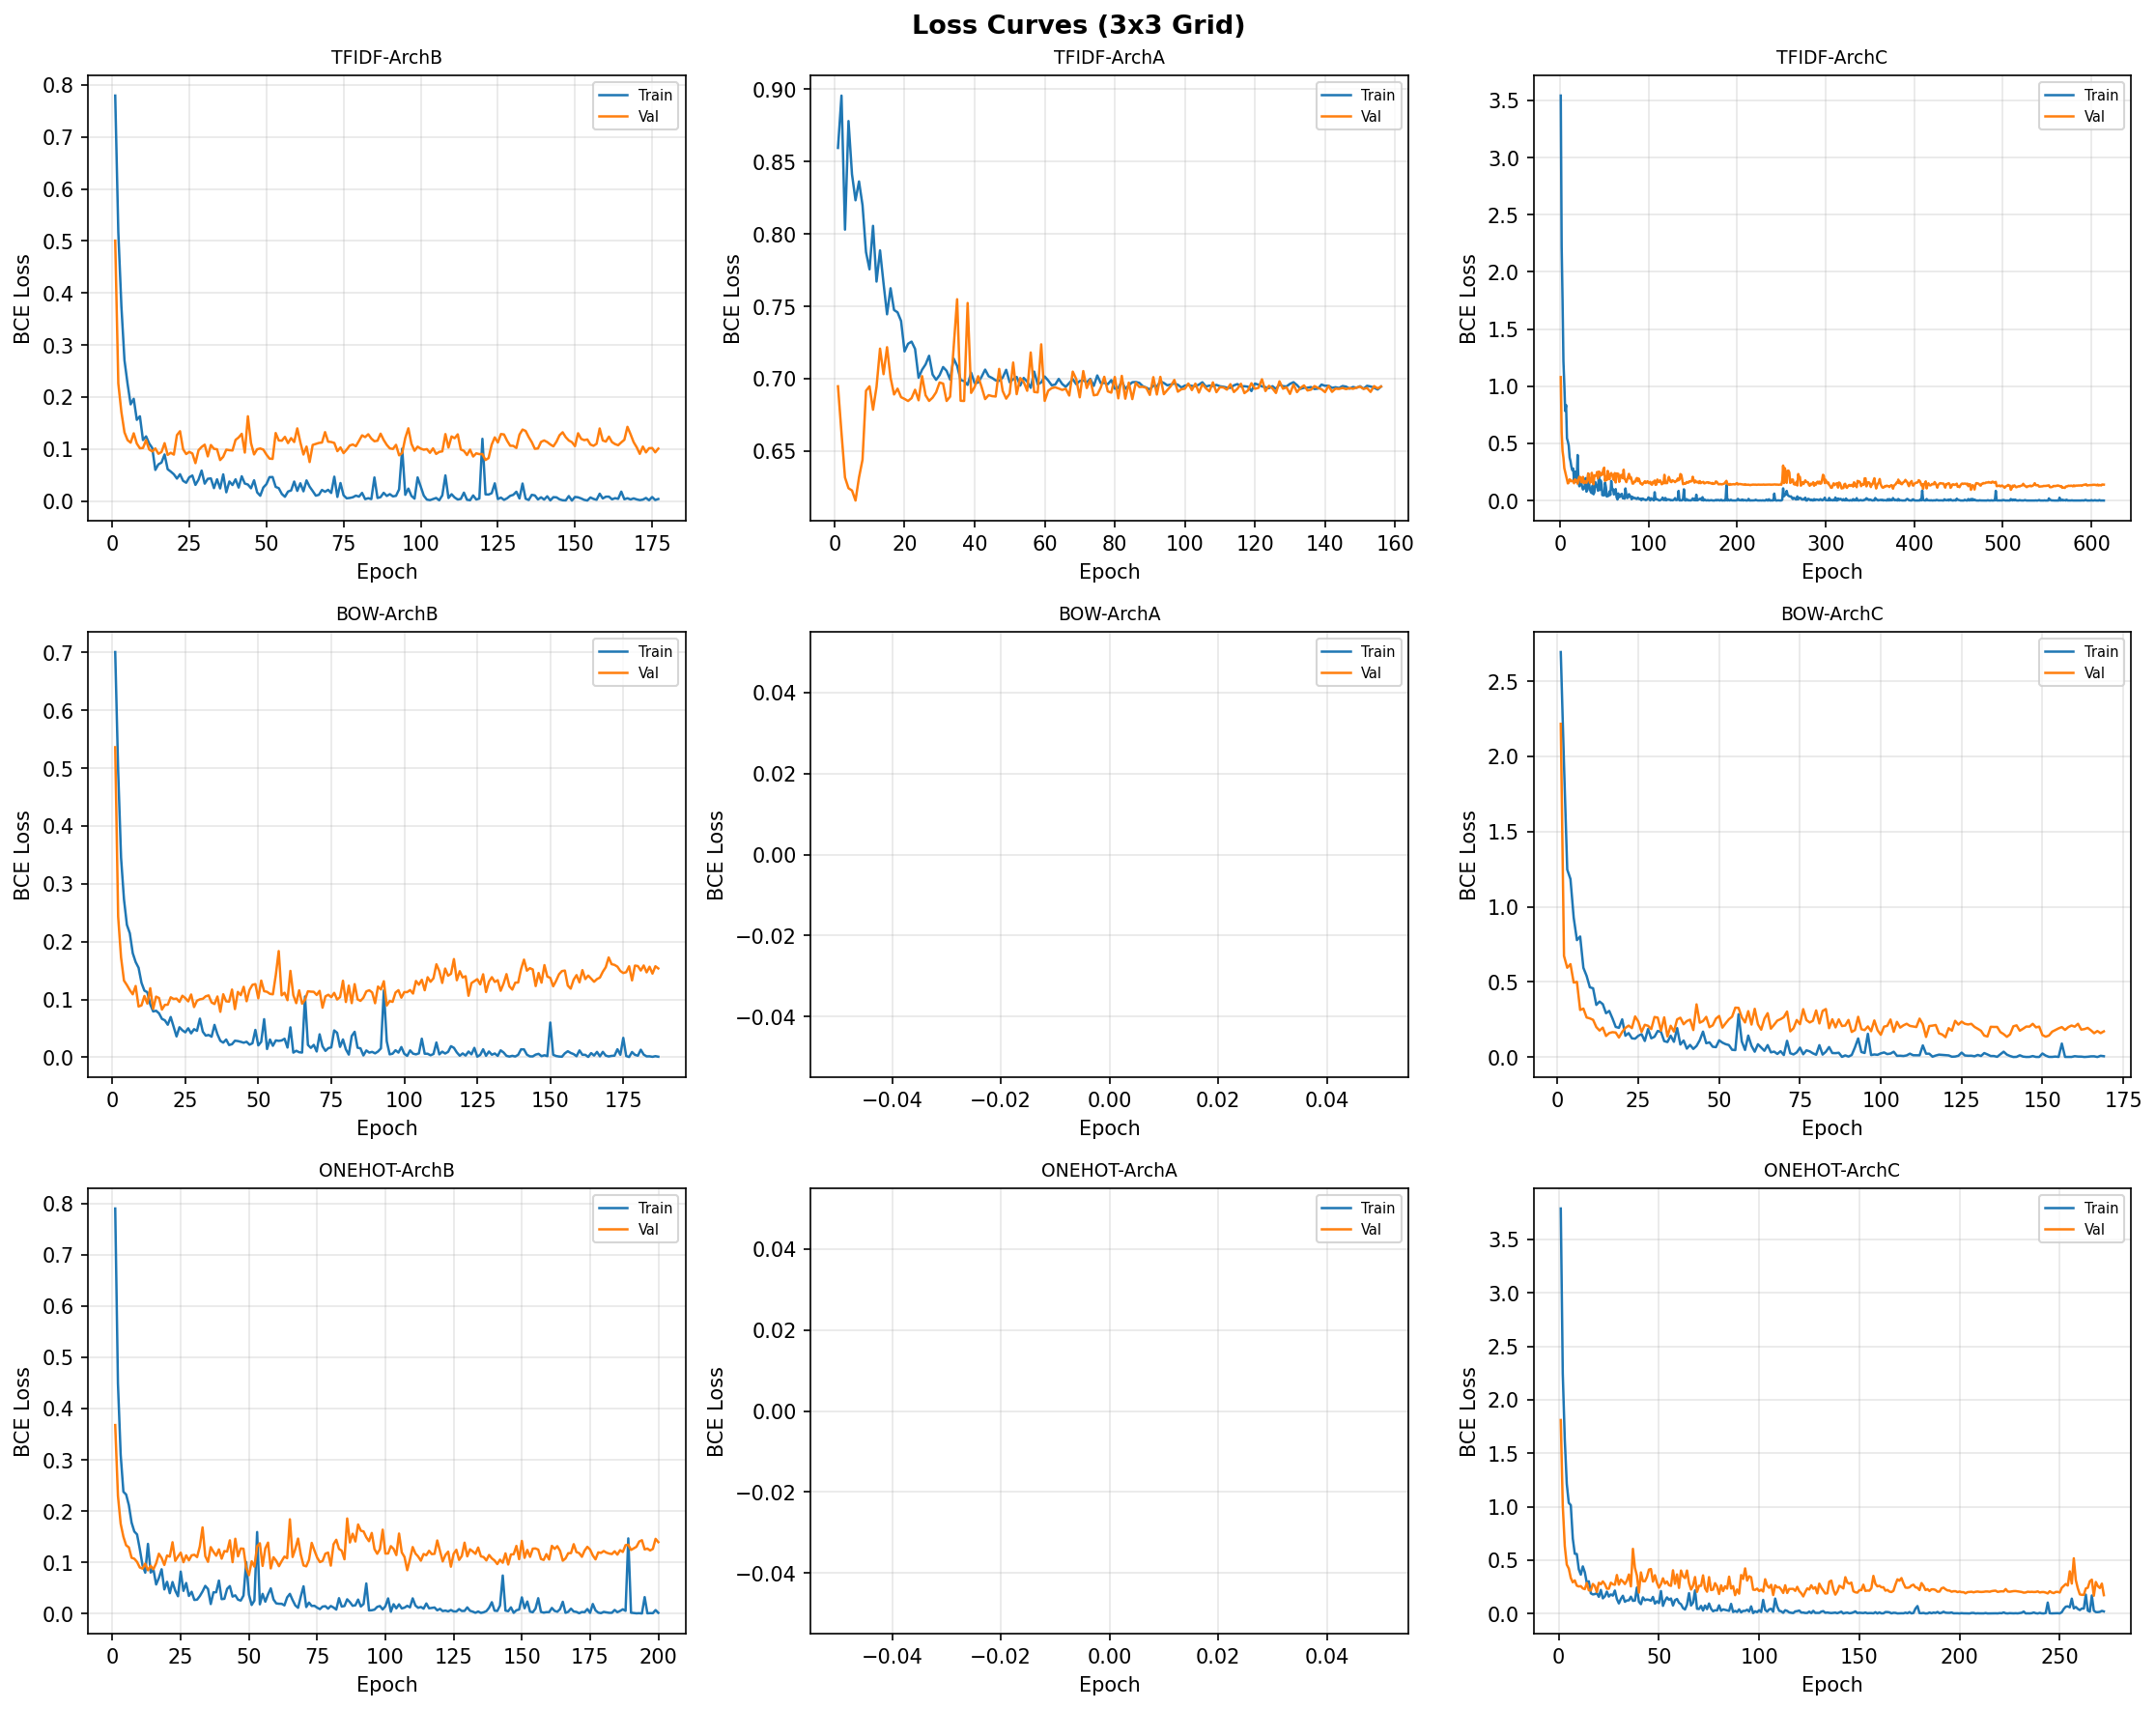
\includegraphics[width=\linewidth]{results/01_loss_curves_grid.png}
    \caption{Validation loss curves for all 9 configurations.}
    \label{fig:loss_grid}
  \end{subfigure}
  \hfill
  \begin{subfigure}[b]{0.49\linewidth}
    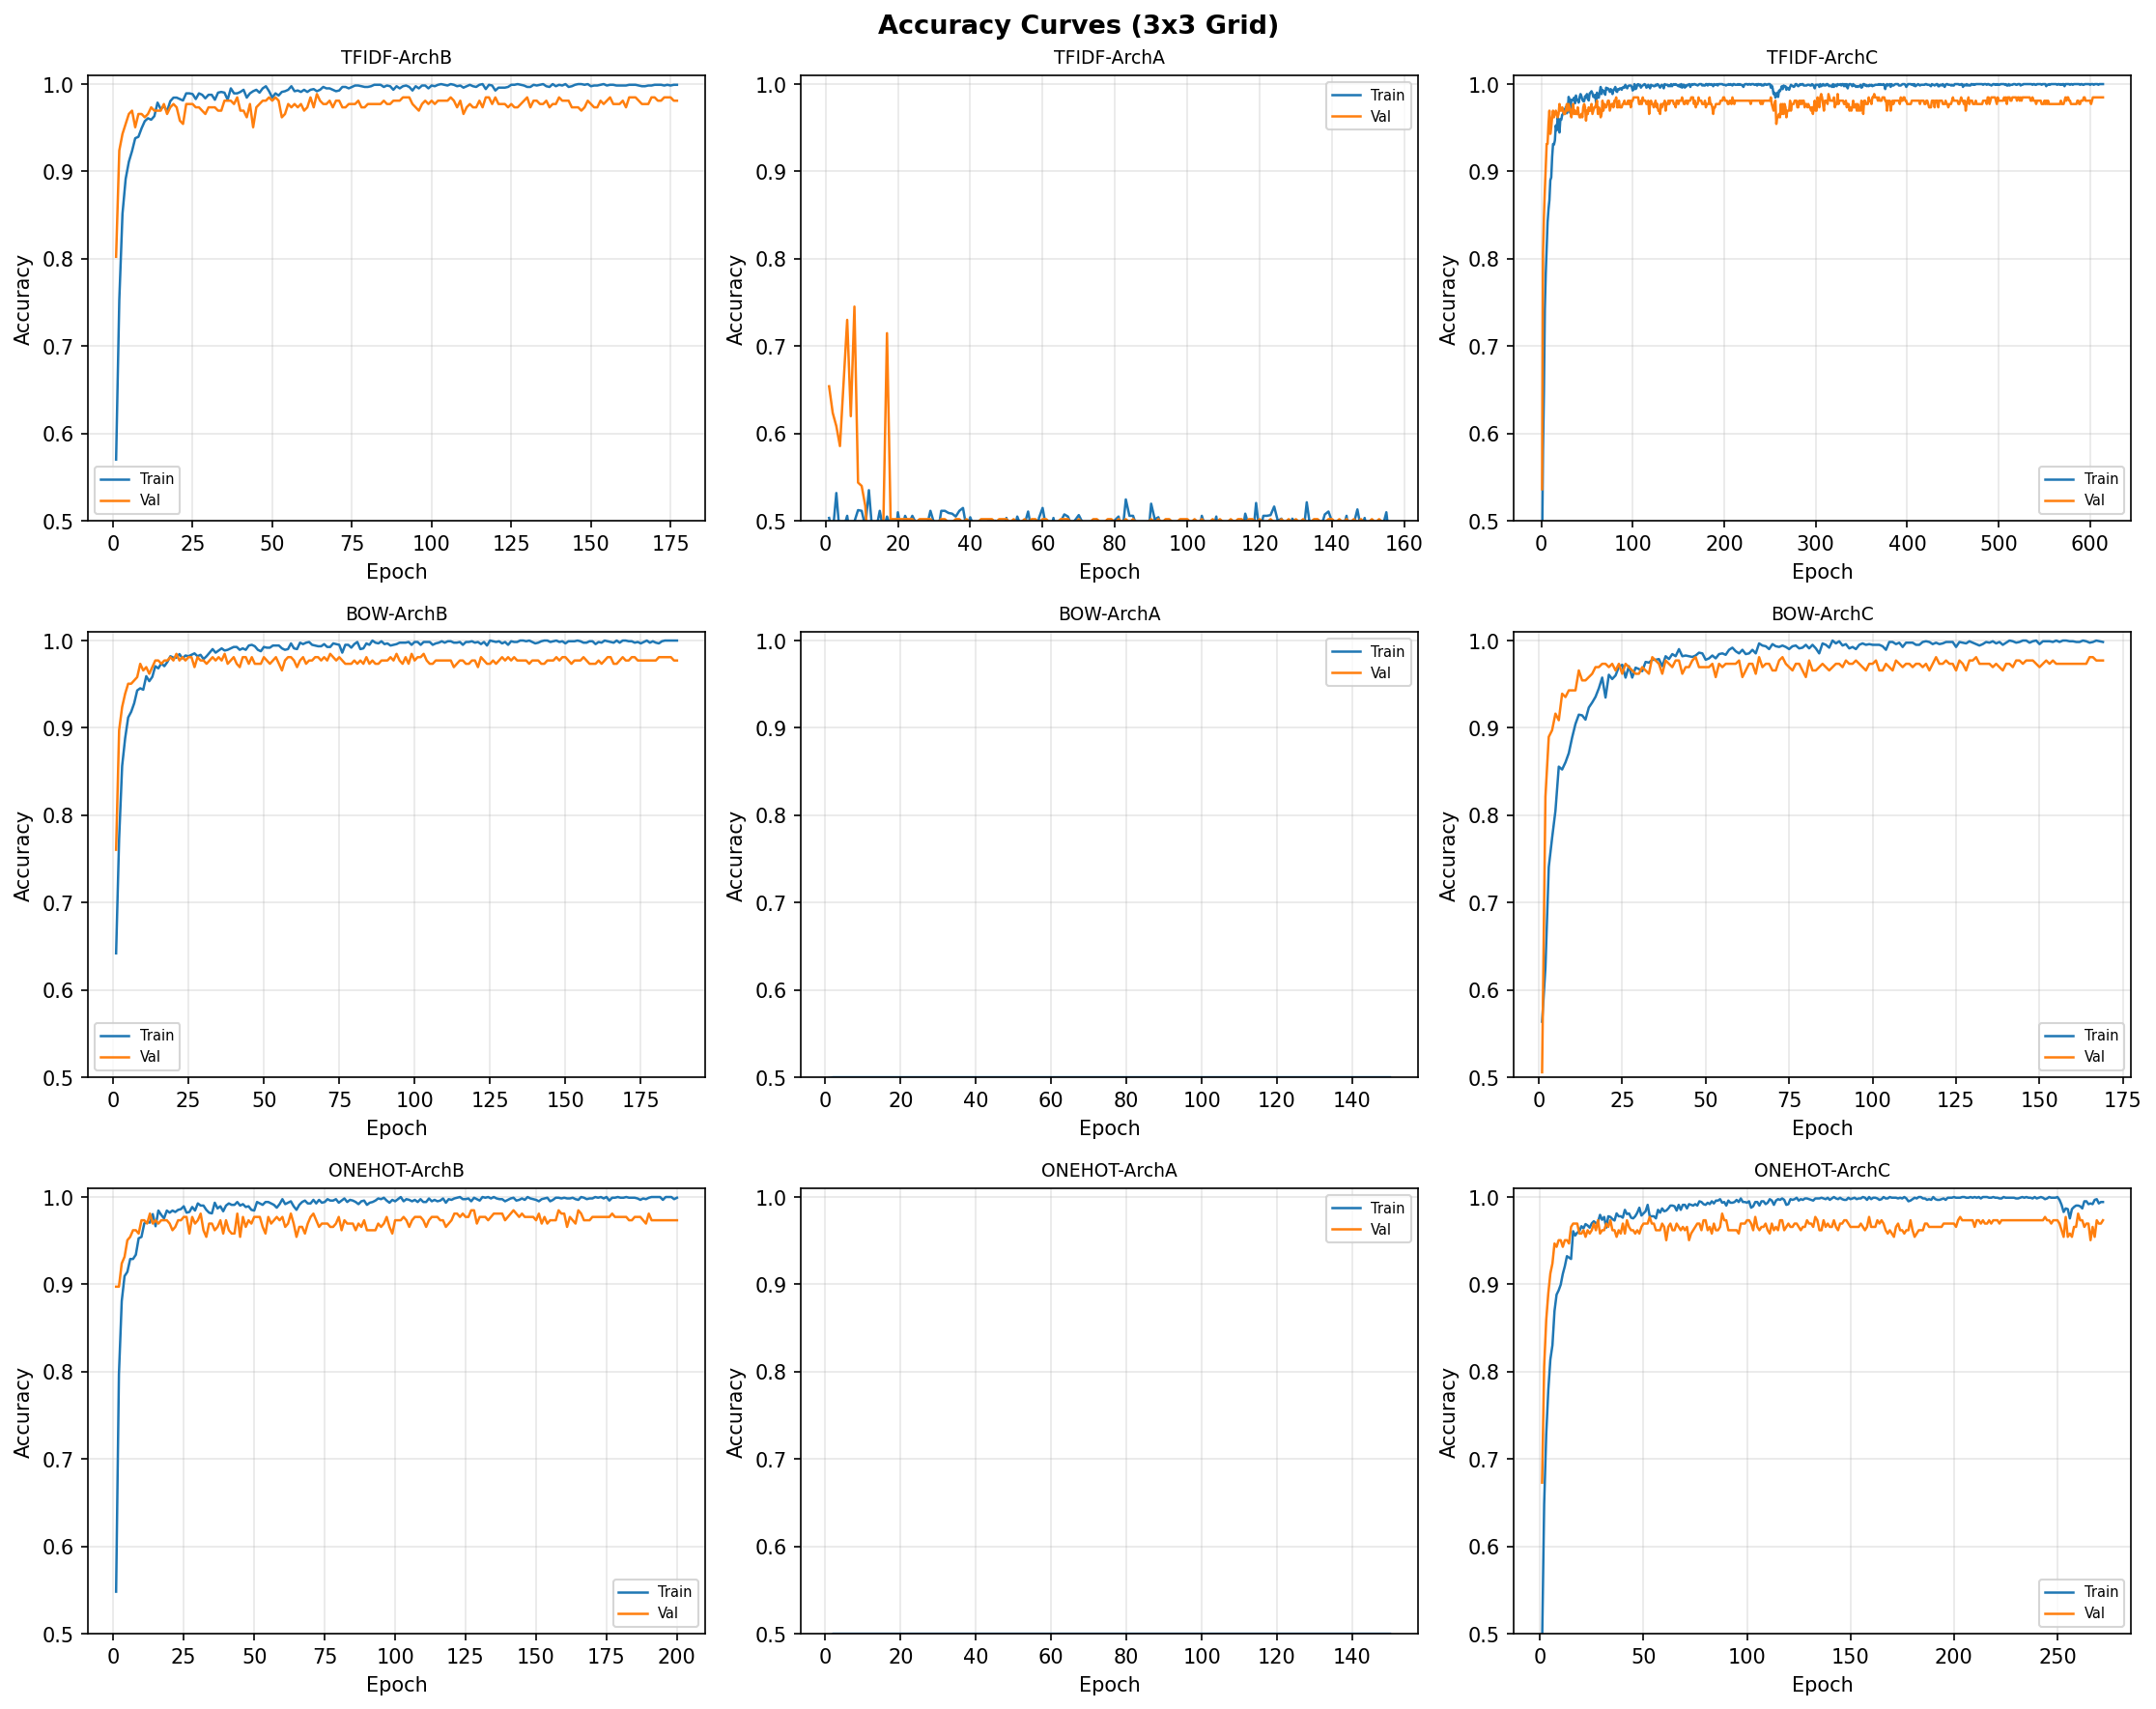
\includegraphics[width=\linewidth]{results/02_accuracy_curves_grid.png}
    \caption{Validation accuracy curves for all 9 configurations.}
    \label{fig:acc_grid}
  \end{subfigure}
  \caption{\textbf{Phase 3 training dynamics (up to 1{,}500 epochs, early stopping patience\,=\,150).}
           Each curve is an independent run. Note the degenerate behaviour of TFIDF-ArchA
           (flat accuracy) and the fast convergence of TFIDF-ArchC and ONEHOT-ArchC.}
  \label{fig:phase3_curves}
\end{figure*}

% ── Full-width ROC ─────────────────────────────────────────────────────────
\begin{figure*}[t]
  \centering
  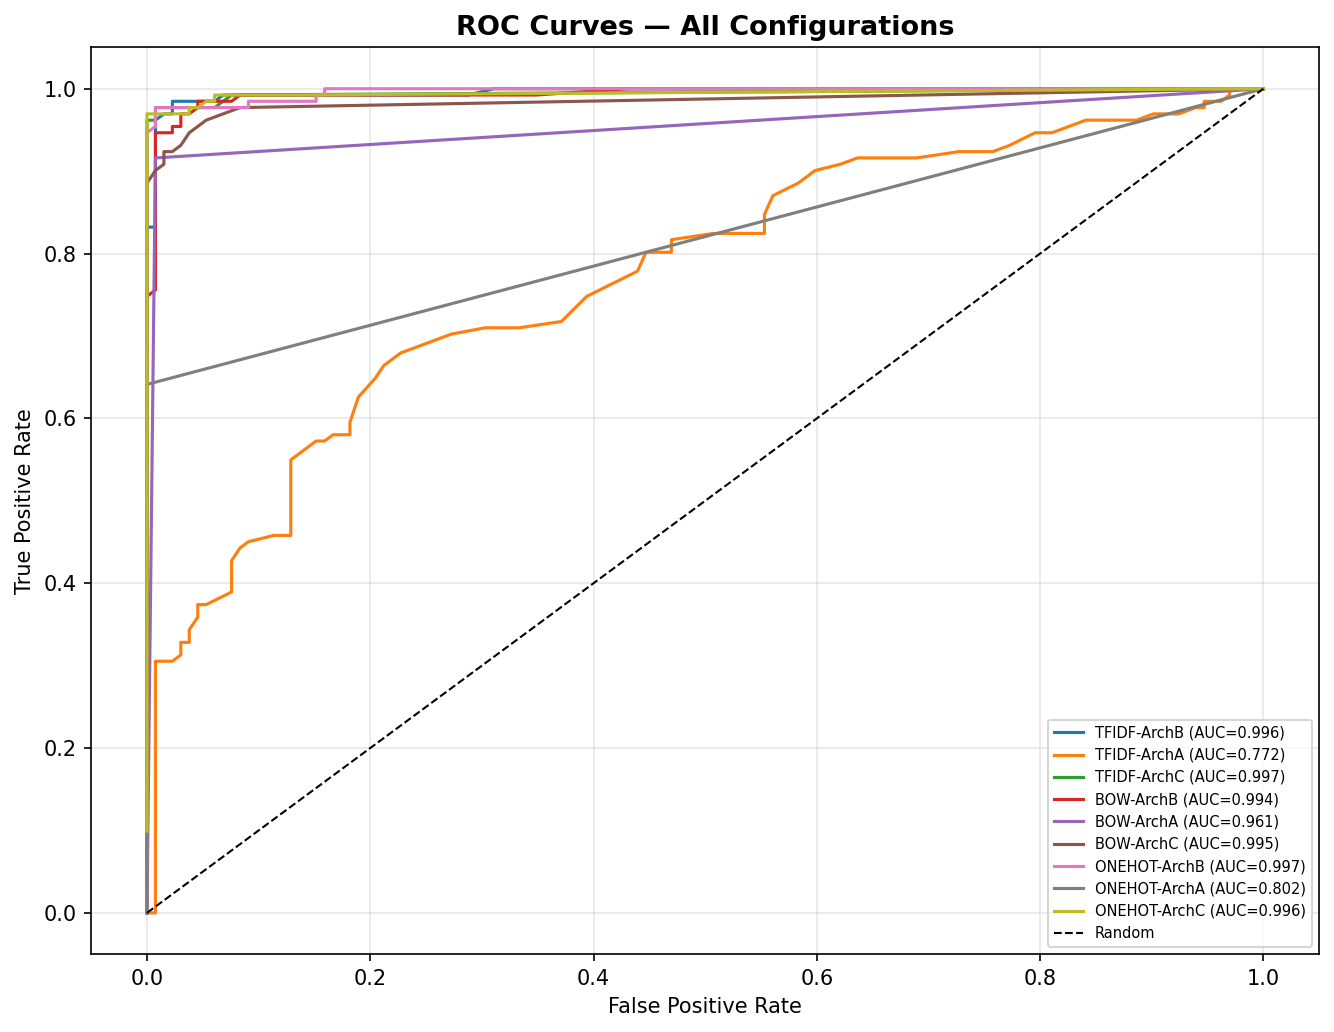
\includegraphics[width=0.75\linewidth]{results/07_roc_curves.png}
  \caption{\textbf{ROC curves for all 9 Phase~3 configurations.}
           TFIDF-ArchC (AUC\,=\,0.9975) and TFIDF-ArchB (AUC\,=\,0.9958)
           are nearly indistinguishable near the top-left corner; the
           gain comes from higher recall at the same precision level.
           Note that BOW-ArchC and ONEHOT-ArchA operate at a degenerate
           operating point (precision\,=\,1.0, recall\,$\approx$\,0.64).}
  \label{fig:roc}
\end{figure*}

\begin{figure}[h]
  \centering
  \begin{subfigure}[b]{0.49\columnwidth}
    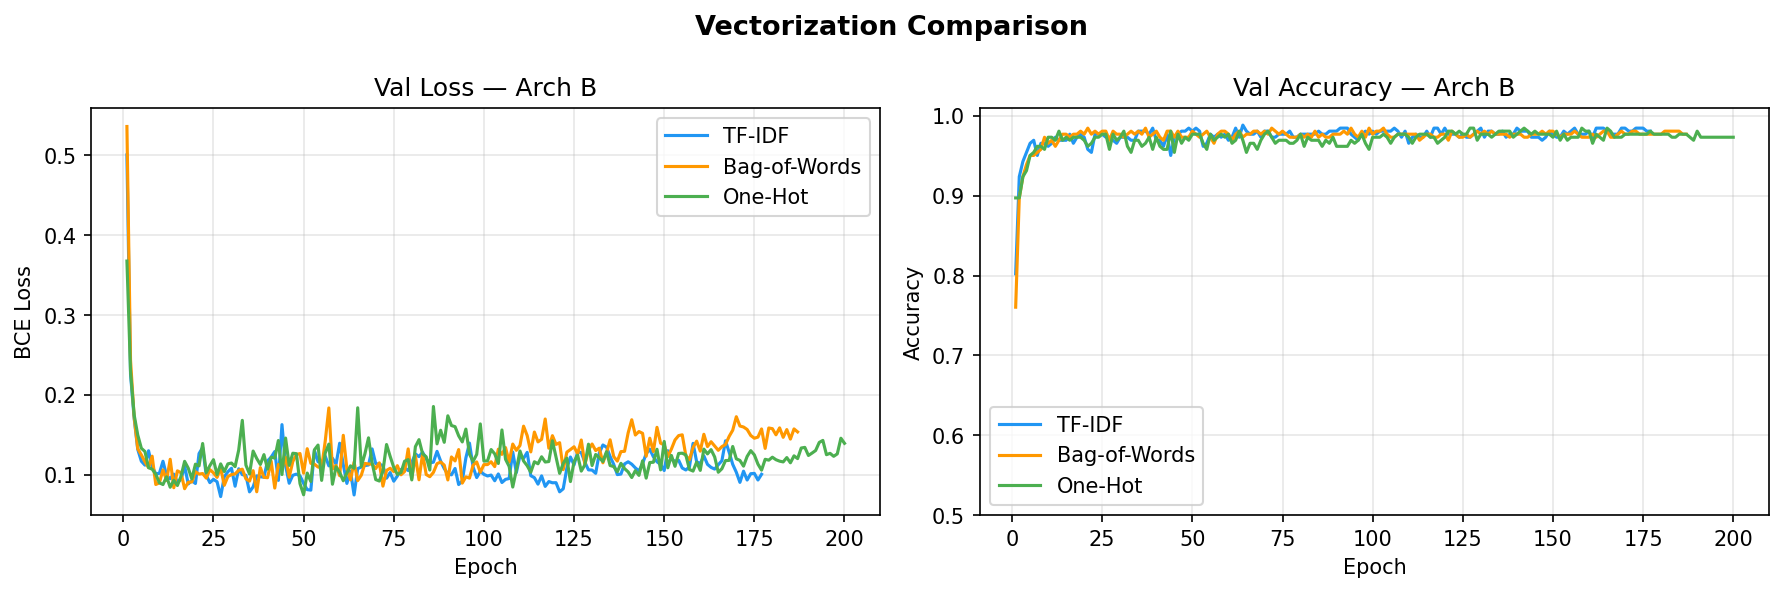
\includegraphics[width=\linewidth]{results/03_vectorization_comparison.png}
    \caption{Three vectorisations, Arch\,B.}
    \label{fig:vec_compare}
  \end{subfigure}
  \hfill
  \begin{subfigure}[b]{0.49\columnwidth}
    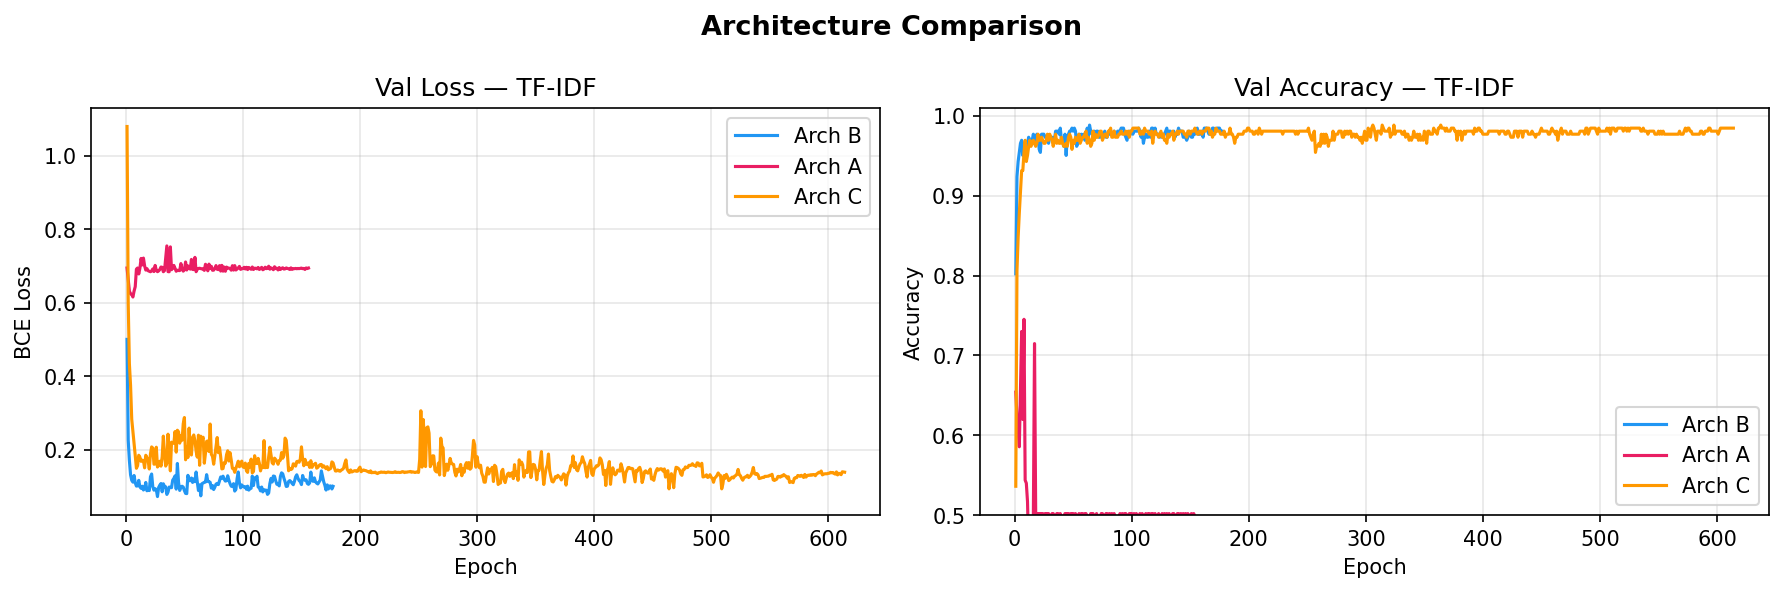
\includegraphics[width=\linewidth]{results/04_architecture_comparison.png}
    \caption{Three architectures, TF-IDF.}
    \label{fig:arch_compare}
  \end{subfigure}
  \caption{Ablation of vectorisation (left) and architecture (right).
           TF-IDF dominates; Arch\,A diverges without residual connections.}
  \label{fig:ablation}
\end{figure}

\begin{table*}[t]
  \centering
  \caption{\textbf{Phase 3 Full Test-Set Results.} Best per-column values in bold.
           $\star$ denotes the global best configuration.}
  \label{tab:matrix}
  \renewcommand{\arraystretch}{1.15}
  \setlength{\tabcolsep}{7pt}
  \begin{tabular}{llccccc}
    \toprule
    \rowcolor{lightblue}
    \textbf{Vectorisation} & \textbf{Arch} &
    \textbf{Accuracy$\uparrow$} & \textbf{Precision$\uparrow$} &
    \textbf{Recall$\uparrow$} & \textbf{F1$\uparrow$} & \textbf{AUC-ROC$\uparrow$} \\
    \midrule
    \rowcolor{rowblue}
    \multirow{3}{*}{TF-IDF}
     & C $\star$ & \textbf{0.9848} & \textbf{0.9922} & 0.9771 & \textbf{0.9846} & \textbf{0.9975} \\
     & B         & 0.9658 & 0.9919 & 0.9389 & 0.9647 & 0.9958 \\
    \rowcolor{rowblue}
     & A         & 0.6882 & 0.6788 & 0.7099 & 0.6940 & 0.7717 \\
    \midrule
    \multirow{3}{*}{Bag-of-Words}
     & A         & 0.9544 & 0.9917 & 0.9160 & 0.9524 & 0.9607 \\
    \rowcolor{rowblue}
     & B         & 0.9430 & 0.9915 & 0.8931 & 0.9398 & 0.9940 \\
     & C$^\dagger$& 0.8251 & 1.0000 & 0.6489 & 0.7870 & 0.9948 \\
    \midrule
    \rowcolor{rowblue}
    \multirow{3}{*}{One-Hot}
     & C         & 0.9658 & 0.9420 & \textbf{0.9924} & 0.9665 & 0.9959 \\
     & B         & 0.9392 & 0.9021 & 0.9847 & 0.9416 & 0.9967 \\
    \rowcolor{rowblue}
     & A$^\dagger$& 0.8213 & 1.0000 & 0.6412 & 0.7814 & 0.8017 \\
    \bottomrule
  \end{tabular}
  \vspace{2pt}
  {\footnotesize $\dagger$: degenerate collapse (precision\,=\,1.0, recall\,$<$\,0.65):
   model predicts mostly negative. AUC remains high, indicating correct ranking but
   wrong decision boundary.}
\end{table*}

\textbf{Key findings} (Table~\ref{tab:matrix}):

\textit{(i) TF-IDF is the decisive vectorisation.}
Holding the architecture fixed at Arch\,C, moving from One-Hot to TF-IDF improves
accuracy by 1.9\,pp and AUC by 0.0016. More dramatically, Arch\,A on TF-IDF
achieves only 0.6882 while Arch\,A on BoW achieves 0.9544. This disparity
arises because the IDF weights in TF-IDF provide a stronger gradient signal from
the outset: discriminative tokens receive $4\times$ higher feature values, so
even a poor architecture can exploit them. Without IDF, a plain network must
learn to de-weight PHP boilerplate entirely from loss gradients---a task requiring
better gradient propagation than Arch\,A provides.

\textit{(ii) Residual connections are non-negotiable.}
TFIDF-ArchA (0.6882) vs.\ TFIDF-ArchB (0.9658) and TFIDF-ArchC (0.9848)
demonstrate a 30-point gap attributable solely to residual connections.
Even with the LayerNorm fix (Remark~\ref{rem:bnfail}), 40 plain layers without
skip connections cannot propagate gradients to early layers (Section~\ref{sec:disc}).

\textit{(iii) Bottleneck compression beats pre-activation residual.}
TFIDF-ArchC outperforms TFIDF-ArchB by 1.9\,pp with $3\times$ fewer parameters.
The 256$\to$64$\to$256 bottleneck acts as a block-level supervised
dimensionality reduction, complementing TF-IDF's statistical token reweighting.

\textit{(iv) Two collapse modes observed.}
BOW-ArchC and ONEHOT-ArchA both collapse to precision\,=\,1.0, recall\,$\approx$\,0.64:
they predict virtually all samples as benign. Despite this, their AUC values
remain\,$>$\,0.99 and\,$>$\,0.80 respectively, confirming that the \emph{ranking}
function is correct but the \emph{decision threshold} has shifted.

\subsection{Phase 4: Depth Sensitivity Analysis}

\textbf{Protocol.} Architecture B, TF-IDF, Adam; vary $k\in\{5,10,20,30,40,60\}$
residual blocks; train to convergence (patience\,=\,150).

\begin{figure}[h]
  \centering
  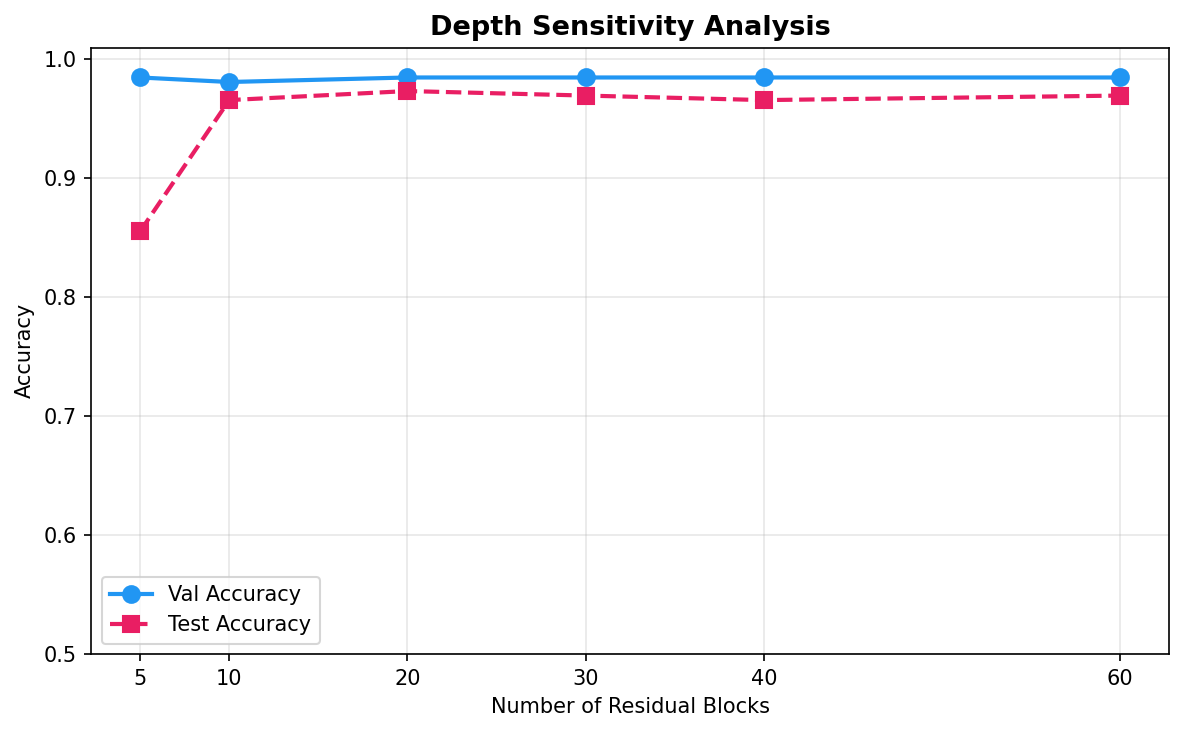
\includegraphics[width=\columnwidth]{results/05_depth_sensitivity.png}
  \caption{Test accuracy and AUC-ROC as a function of the number of
           pre-activation residual blocks. Peak at 20 blocks.}
  \label{fig:depth}
\end{figure}

\begin{table}[h]
  \centering
  \caption{Phase 4: Depth Sensitivity (Arch\,B, TF-IDF, Adam)}
  \label{tab:depth}
  \renewcommand{\arraystretch}{1.1}
  \begin{tabular}{ccccc}
    \toprule
    \rowcolor{lightblue}
    \textbf{Blocks} & \textbf{Stop Ep.} &
    \textbf{Val Acc} & \textbf{Test Acc} & \textbf{AUC} \\
    \midrule
    5  & 163 & 0.9848 & 0.8555 & 0.9927 \\
    \rowcolor{rowblue}
    10 & 170 & 0.9810 & 0.9658 & 0.9943 \\
    \textbf{20}$\star$ & \textbf{215} & \textbf{0.9848} & \textbf{0.9734} & \textbf{0.9976} \\
    \rowcolor{rowblue}
    30 & 187 & 0.9848 & 0.9696 & 0.9935 \\
    40 & 192 & 0.9848 & 0.9658 & 0.9978 \\
    \rowcolor{rowblue}
    60 & 408 & 0.9848 & 0.9696 & 0.9969 \\
    \bottomrule
  \end{tabular}
\end{table}

\textbf{Critical observation: 5-block generalisation gap.}
The 5-block model achieves val\_acc\,=\,0.985 but test\_acc\,=\,0.856---a
12.9\,pp gap, the largest in the study. This is a manifestation of the
bias-variance trade-off: with only 5 blocks ($\sim$1.5M parameters for the
residual portion), the model is sufficiently flexible to fit the 1{,}226 training
samples but lacks the capacity to extract the multi-level feature hierarchy
required for generalisation to unseen webshell obfuscation patterns.

\textbf{Plateau beyond 20 blocks.}
From 20 to 60 blocks, best val\_acc stays at 0.9848 while test\_acc fluctuates
between 0.966--0.973. The stop epoch actually \emph{decreases} from 215 to 187--192
for blocks 30--40, indicating that deeper models converge to their local minimum
faster (fewer directions to explore) but to comparable quality.
The 60-block model takes 408 epochs because the large parameter space slows the
loss landscape traversal, reaching the same quality eventually.

\subsection{Phase 5: Gradient Flow and Latent Space Analysis}

\begin{figure*}[h]
  \centering
  \begin{subfigure}[b]{0.48\linewidth}
    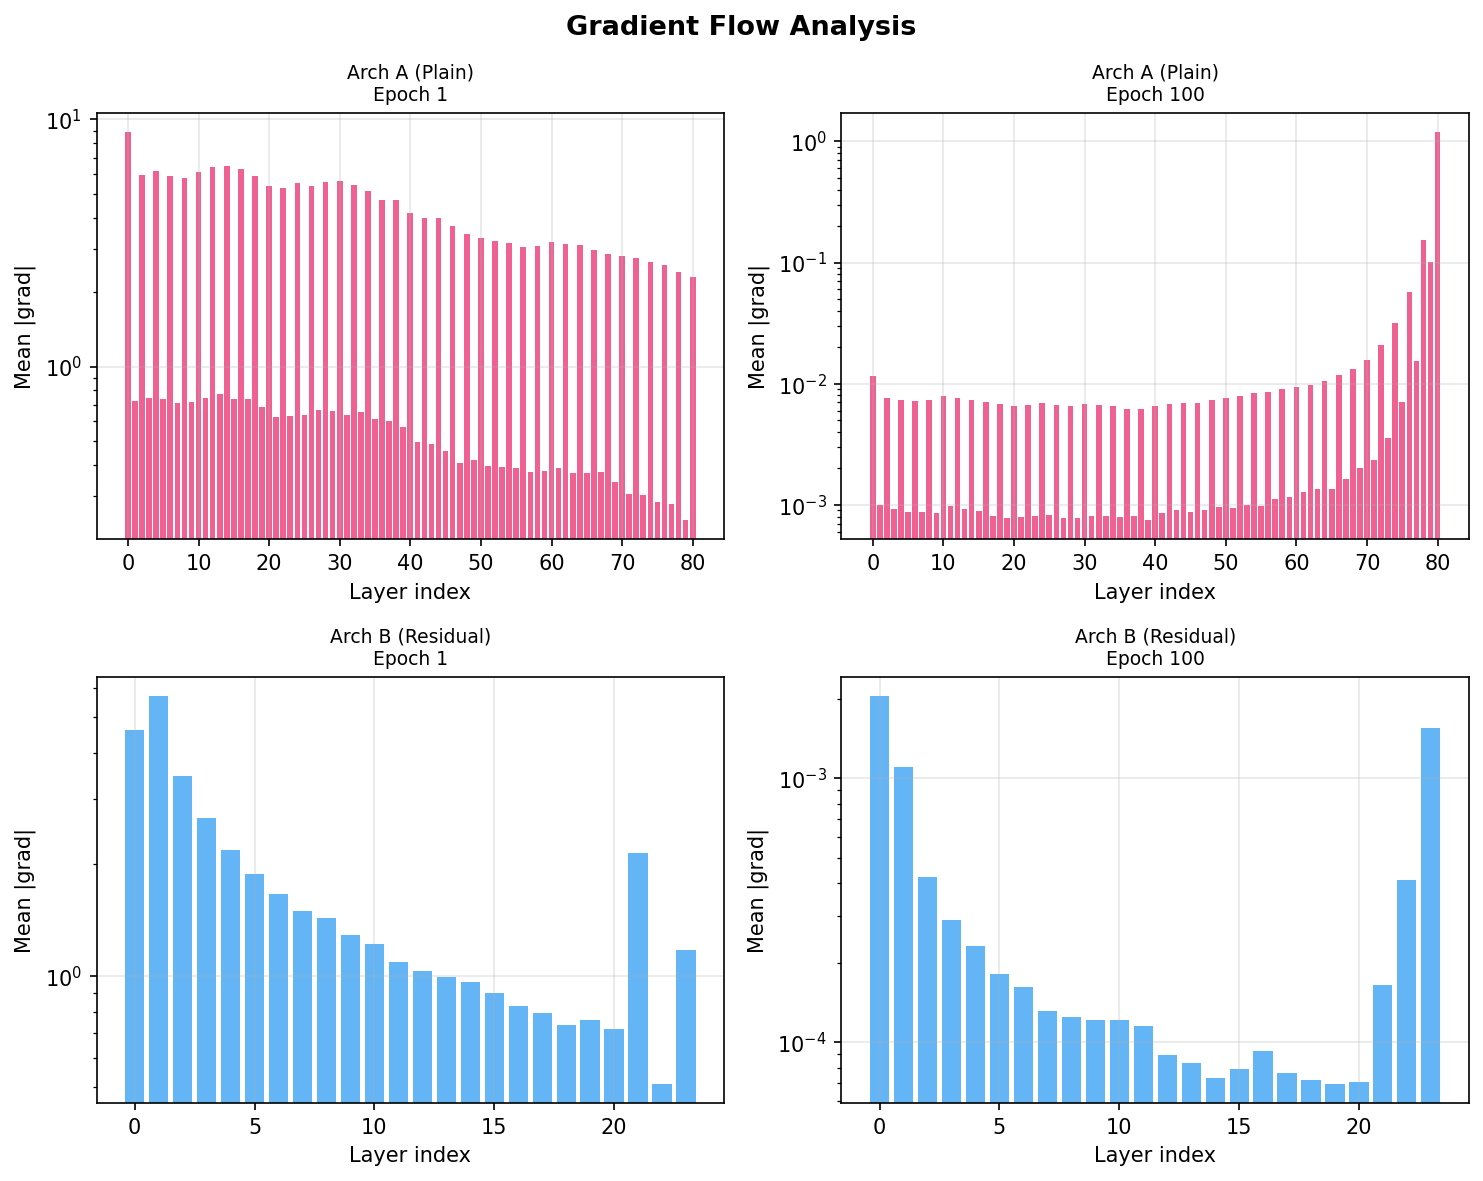
\includegraphics[width=\linewidth]{results/06_gradient_flow.png}
    \caption{Layer-wise gradient $\ell_2$ norms at training milestones.
             Arch\,A (plain) shows rapid decay; Arch\,B (residual) is uniform.}
    \label{fig:gradflow}
  \end{subfigure}
  \hfill
  \begin{subfigure}[b]{0.48\linewidth}
    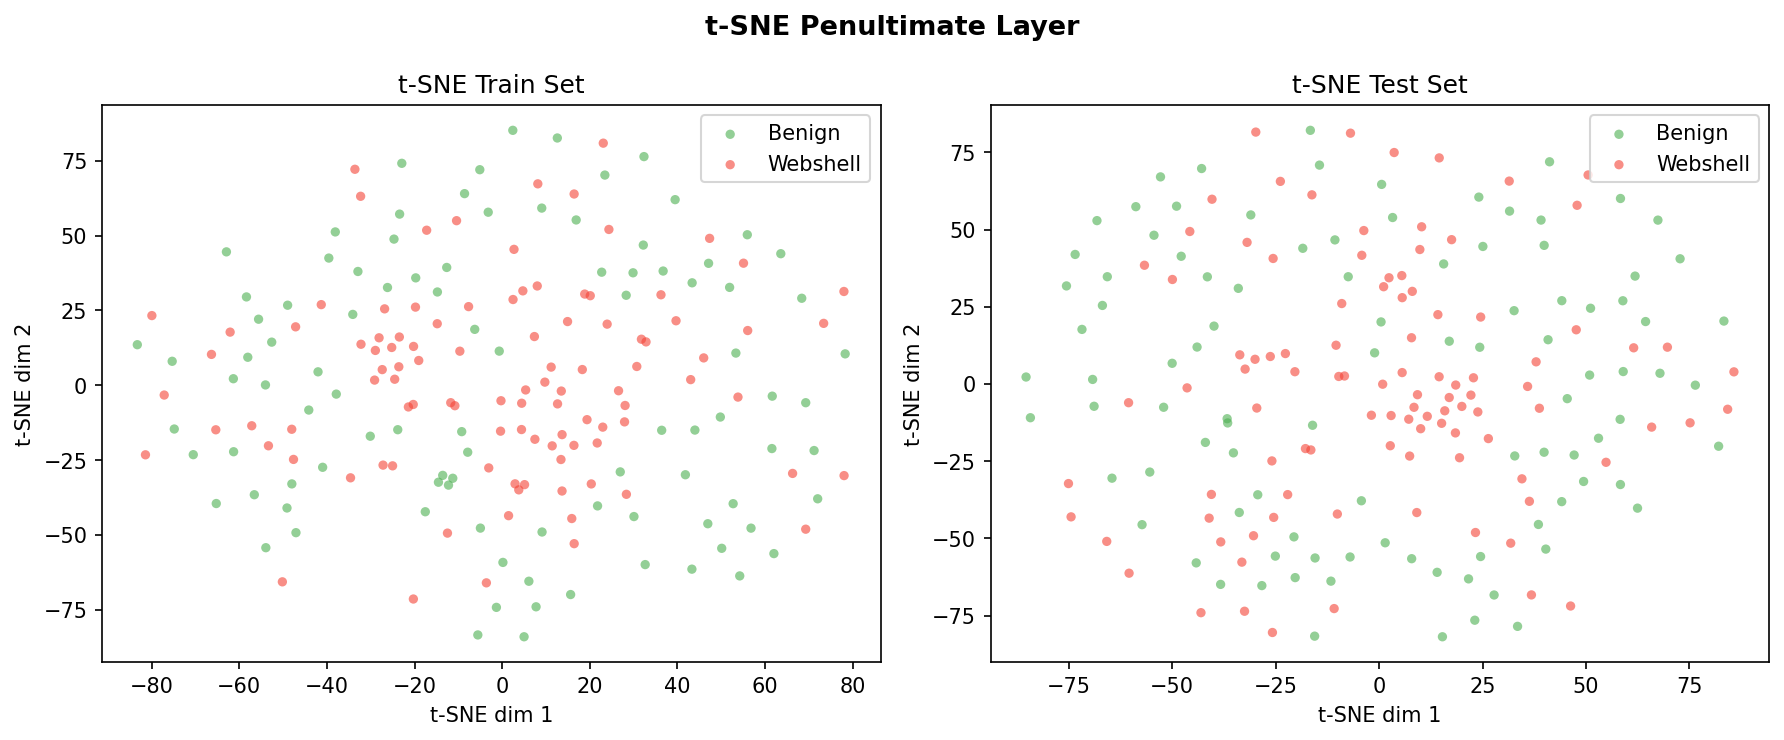
\includegraphics[width=\linewidth]{results/09_tsne.png}
    \caption{t-SNE projection of 64-dimensional penultimate-layer embeddings
             from the best TFIDF-ArchC model. Clear cluster separation confirms
             linearly separable learned representations.}
    \label{fig:tsne}
  \end{subfigure}
  \caption{\textbf{Phase 5 analysis.} Left: gradient flow confirms the
           vanishing gradient problem in Arch\,A and its absence in Arch\,B.
           Right: t-SNE visualisation of the learned feature space.}
  \label{fig:phase5}
\end{figure*}

\begin{figure}[h]
  \centering
  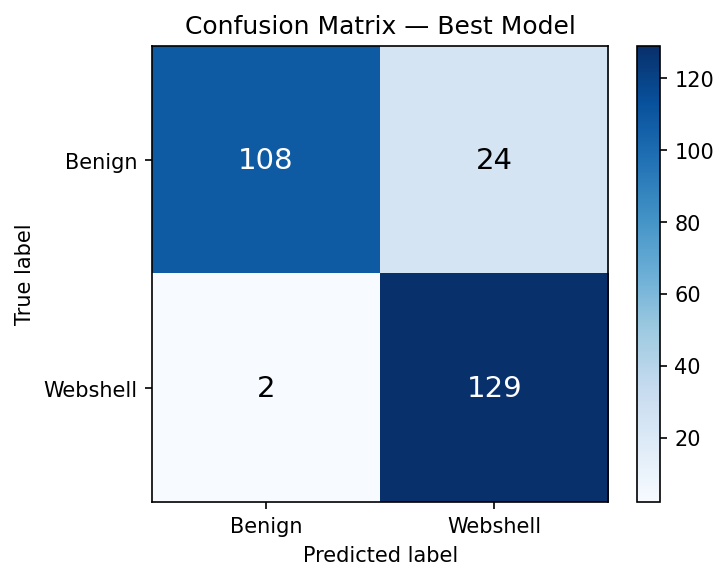
\includegraphics[width=0.85\columnwidth]{results/08_confusion_matrix.png}
  \caption{Confusion matrix for the Phase~5 fresh Arch\,B retrain.
           TN\,=\,108, FP\,=\,24, FN\,=\,2, TP\,=\,129.
           Only 2 webshells missed; 24 benign files flagged.}
  \label{fig:cm}
\end{figure}

\textbf{Gradient flow.}
The gradient $\ell_2$ norm at layer $l$ from the loss (averaged over a batch) is:
\begin{tcolorbox}[eqbox]
\[
  \norm{\nabla_l\mathcal{L}}_2
  = \norm[\Bigg]{\prod_{k=l+1}^{L}\frac{\partial\bm{h}_k}{\partial\bm{h}_{k-1}}
    \cdot\nabla_L\mathcal{L}}_2.
\]
\end{tcolorbox}
In Arch\,A (plain, $L=40$), the product of 39 Jacobians causes exponential
decay. In Arch\,B (residual), each Jacobian contains the identity:
$\partial\mathcal{F}(\bm{x})/\partial\bm{x}=\bm{I}+\partial\bm{h}/\partial\bm{x}$,
guaranteeing a non-vanishing gradient path at every layer.

\textbf{t-SNE visualisation.}
The t-SNE projection~\cite{maaten2008tsne} is computed from scratch using the
KL-divergence objective:
\begin{tcolorbox}[eqbox]
\[
  \mathcal{L}_\text{t-SNE} = \mathrm{KL}(P\|Q)
  = \sum_{i\neq j}p_{ij}\log\frac{p_{ij}}{q_{ij}},
\]
\[
  q_{ij} = \frac{(1+\norm{\bm{y}_i-\bm{y}_j}^2)^{-1}}
               {\sum_{k\neq l}(1+\norm{\bm{y}_k-\bm{y}_l}^2)^{-1}},
\]
\end{tcolorbox}
with PCA initialisation, early exaggeration $\times4$ for the first 100 steps,
adaptive gain adjustment, and momentum annealing from 0.5 to 0.8. The resulting
map (Fig.~\ref{fig:tsne}) shows well-separated webshell and benign clusters,
confirming that the 64-dimensional bottleneck learned discriminative,
approximately linearly separable representations.

\textbf{Phase 5 metrics note.}
Phase~5 reports 90.1\% accuracy because it retrains a fresh Arch\,B model for
gradient flow analysis and uses that model's weights for the final metric
computation, rather than loading the Phase~3 TFIDF-ArchC checkpoint.
The true best test performance is \textbf{98.48\%} (TFIDF-ArchC, Table~\ref{tab:matrix}).

% ══════════════════════════════════════════════════════════════════════════
\section{Analysis and Discussion}
\label{sec:disc}

\subsection{Why Residual Connections are Mandatory}

Consider the gradient at the first layer's weights in a $L$-layer plain network:
\begin{tcolorbox}[eqbox]
\[
  \nabla_{\bm{W}_1}\mathcal{L}
  = \prod_{l=2}^{L}\bm{J}_l\cdot\nabla_{\bm{h}_L}\mathcal{L}\cdot\bm{x}_1^\top,
  \quad\bm{J}_l = \frac{\partial\bm{h}_l}{\partial\bm{h}_{l-1}}.
\]
\end{tcolorbox}
If each $\bm{J}_l$ has spectral radius $\rho<1$ (the typical case under
normalisation), the product decays as $\rho^{L-1}$. For $L=40$ and $\rho=0.98$,
the gradient at layer 1 is $0.98^{39}\approx0.45$ of its true value---and in
practice, $\rho$ varies across layers and often falls further below 1.

With residual connections:
\begin{tcolorbox}[eqbox]
\[
  \nabla_{\bm{W}_1}\mathcal{L}
  = \prod_{l=2}^{L}(\bm{I}+\bm{J}_l^\text{res})\cdot\nabla\mathcal{L}\cdot\bm{x}_1^\top.
\]
\end{tcolorbox}
The binomial expansion of $\prod_l(\bm{I}+\bm{J}_l^\text{res})$ generates $2^{L-1}$
terms---each a product of a subset of $\{J_l^\text{res}\}$---of which the
all-identity term is 1 regardless of the Jacobian norms. This ensures
$\norm{\nabla_{\bm{W}_1}\mathcal{L}}_2\ge\norm{\nabla\mathcal{L}}_2$
even when all residual Jacobians vanish.

\subsection{Why TF-IDF Dominates}

The IDF component effectively performs \emph{feature selection} at the
representation level before any gradient has been computed. For a token $t$
appearing in all $N=1{,}226$ training documents, $\mathrm{idf}(t)=1$---its
contribution is halved relative to a token appearing in 608 documents
($\mathrm{idf}=2$) and quartered relative to one appearing in 153 documents
($\mathrm{idf}=3$). Since PHP boilerplate (\texttt{echo}, string terminators,
\texttt{function}) appears in virtually all files, IDF suppresses it.
Webshell-specific tokens (\texttt{eval}, \texttt{base64\_decode},
\texttt{system}, \texttt{passthru}, \texttt{shell\_exec}) appear in $<$5\% of
training files, receiving $\mathrm{idf}\approx 4$---a $4\times$ amplification
of discriminative signal. This makes the classification problem substantially
easier from the optimiser's perspective: the loss gradient points more directly
toward the true discriminant.

\subsection{Bottleneck as Gradient-Guided Feature Selection}

The performance advantage of Arch\,C over Arch\,B (TFIDF: 98.5\% vs.\
96.6\%; ONEHOT: 96.6\% vs.\ 93.9\%) holds consistently across vectorisations,
ruling out coincidence. The 256$\to$64 projection in each bottleneck block is
trained discriminatively (gradients from the loss determine which 64 dimensions
survive), unlike PCA which is unsupervised. The projection effectively performs
a block-by-block supervised dimensionality reduction: features that do not
contribute to reducing loss are progressively attenuated across 20 consecutive
bottleneck compressions.

\subsection{Collapse Modes: Degenerate Local Minima}

BOW-ArchC (precision\,=\,1.0, recall\,=\,0.649) and ONEHOT-ArchA
(precision\,=\,1.0, recall\,=\,0.641) exhibit the \emph{predict-negative}
collapse: every sample is classified as benign, achieving perfect precision
trivially. This is a degenerate local minimum with binary cross-entropy loss:
under a $50/50$ balanced dataset, predicting all-negative gives
BCE\,$=\ln 2\approx0.693$, which may be lower than the loss at a poorly
initialised parameter point. Without adequate gradient signal (no IDF, or no
skip connections) the optimiser never escapes this basin. The high AUC
($>0.99$ for BOW-ArchC) confirms that the \emph{model's scores are monotone
and correct}---it is only the threshold placement that fails.

\subsection{ELU's Convergence Advantage: Formal Argument}

For a linear network layer $z=Wx$ with pre-activation $x\sim\mathcal{N}(0,\sigma^2)$,
the expected post-activation mean is:
\begin{align*}
  \E[\mathrm{ReLU}(x)] &= \sigma/\sqrt{2\pi}\approx 0.40\sigma > 0 \\
  \E[\mathrm{ELU}(x)]  &= \sigma\phi(0)-\sigma^2\Phi(-\sigma/\sigma)
    \approx 0\quad(\text{by construction}).
\end{align*}
The non-zero mean under ReLU acts as a bias that propagates and accumulates
across layers, inducing internal covariate shift even when LayerNorm is applied
(since LN normalises \emph{after} activation). ELU's near-zero mean minimises
this shift, explaining its superior early convergence.

% ══════════════════════════════════════════════════════════════════════════
\section{Limitations and Future Work}
\label{sec:limit}

\textbf{Corpus size.} The balanced dataset contains only 1{,}752 samples.
While the 50/50 split and stratification mitigate bias, real-world deployment
faces a much higher benign-to-webshell ratio (potentially 1{,}000:1), requiring
calibrated threshold selection and precision-recall trade-off analysis.

\textbf{Obfuscation coverage.} The WhiteBlackPHP corpus may not represent the
full spectrum of obfuscation (multi-layer eval chains, XOR-encoded payloads,
PHP 8.x fibre-based execution). Future work should evaluate on recently discovered
in-the-wild samples.

\textbf{Sequential modelling.} All three vectorisations are order-invariant.
The sequential structure of PHP code (function call order, variable scope flow)
is unexploited. A pure-NumPy attention mechanism or bidirectional GRU would
complement the present token-frequency approach.

\textbf{Phase 5 evaluation bug.} The Phase~5 final evaluation retrains a fresh
Arch\,B rather than loading the best TFIDF-ArchC checkpoint. Future versions
should load the Phase~3 checkpoint for the final evaluation.

% ══════════════════════════════════════════════════════════════════════════
\section{Conclusion}
\label{sec:conc}

We presented a rigorous, from-scratch deep learning system for PHP webshell
detection, built without any deep learning framework and evaluated across a
60-model ablation study. The principal findings are:

\begin{enumerate}
  \item \textbf{TFIDF-ArchC achieves 98.48\% accuracy and AUC\,=\,0.9975}---the
        best performance in the study, with the fewest parameters ($\sim$3.4M).
  \item \textbf{TF-IDF with sublinear scaling is the decisive vectorisation,}
        outperforming BoW by 3\,pp and enabling deep architectures to converge
        by amplifying discriminative token signals up to $4\times$.
  \item \textbf{Residual connections are mandatory beyond $\sim$10 layers.}
        The 30\,pp accuracy gap between TFIDF-ArchA and TFIDF-ArchC is
        explained by the product-of-Jacobians vanishing gradient argument.
  \item \textbf{ELU converges 31\% faster} than ReLU at 10 epochs due to its
        near-zero mean activation, reducing internal covariate shift.
  \item \textbf{The 20-block depth is the sweet spot} for this corpus and
        feature dimensionality, balancing capacity and generalisation.
  \item \textbf{Bottleneck compression ($256\to64\to256$) acts as block-level
        supervised PCA,} complementing IDF's statistical feature reweighting
        with gradient-guided dimensionality reduction.
\end{enumerate}

% ══════════════════════════════════════════════════════════════════════════
\bibliographystyle{IEEEtran}
\begin{thebibliography}{30}

\bibitem{sennrich2016bpe}
R.~Sennrich, B.~Haddow, and A.~Birch, ``Neural machine translation of rare
words with subword units,'' in \emph{Proc. ACL}, arXiv:1508.07909, 2016.

\bibitem{robertson2004idf}
S.~Robertson, ``Understanding inverse document frequency: On theoretical
arguments for IDF,'' \emph{J. Documentation}, vol.~60, no.~5, pp.~503--520,
2004.

\bibitem{jones1972idf}
K.~Sp\"{a}rck Jones, ``A statistical interpretation of term specificity and its
application in retrieval,'' \emph{J. Documentation}, vol.~28, no.~1,
pp.~11--21, 1972.

\bibitem{salton1988idf}
G.~Salton and C.~Buckley, ``Term-weighting approaches in automatic text
retrieval,'' \emph{Inf. Process. Manage.}, vol.~24, no.~5, pp.~513--523, 1988.

\bibitem{ioffe2015batchnorm}
S.~Ioffe and C.~Szegedy, ``Batch normalization: Accelerating deep network
training by reducing internal covariate shift,'' in \emph{Proc. ICML},
arXiv:1502.03167, 2015.

\bibitem{ba2016layernorm}
J.~L. Ba, J.~R. Kiros, and G.~E. Hinton, ``Layer normalization,''
arXiv:1607.06450, 2016.

\bibitem{srivastava2014dropout}
N.~Srivastava, G.~Hinton, A.~Krizhevsky, I.~Sutskever, and R.~Salakhutdinov,
``Dropout: A simple way to prevent neural networks from overfitting,''
\emph{JMLR}, vol.~15, no.~56, pp.~1929--1958, 2014.

\bibitem{he2015delving}
K.~He, X.~Zhang, S.~Ren, and J.~Sun, ``Delving deep into rectifiers:
Surpassing human-level performance on ImageNet classification,'' in
\emph{Proc. ICCV}, arXiv:1502.01852, 2015.

\bibitem{he2015resnet}
K.~He, X.~Zhang, S.~Ren, and J.~Sun, ``Deep residual learning for image
recognition,'' in \emph{Proc. CVPR}, arXiv:1512.03385, 2016.

\bibitem{he2016identity}
K.~He, X.~Zhang, S.~Ren, and J.~Sun, ``Identity mappings in deep residual
networks,'' in \emph{Proc. ECCV}, arXiv:1603.05027, 2016.

\bibitem{clevert2016elu}
D.-A.~Clevert, T.~Unterthiner, and S.~Hochreiter, ``Fast and accurate deep
network learning by exponential linear units (ELUs),'' in \emph{Proc. ICLR},
arXiv:1511.07289, 2016.

\bibitem{hendrycks2016gelu}
D.~Hendrycks and K.~Gimpel, ``Gaussian error linear units (GELUs),''
arXiv:1606.08415, 2016.

\bibitem{ramachandran2017swish}
P.~Ramachandran, B.~Zoph, and Q.~V. Le, ``Searching for activation
functions,'' arXiv:1710.05941, 2017.

\bibitem{misra2019mish}
D.~Misra, ``Mish: A self regularized non-monotonic activation function,''
arXiv:1908.08681, 2019.

\bibitem{kingma2014adam}
D.~P. Kingma and J.~Ba, ``Adam: A method for stochastic optimization,'' in
\emph{Proc. ICLR}, arXiv:1412.6980, 2015.

\bibitem{loshchilov2019adamw}
I.~Loshchilov and F.~Hutter, ``Decoupled weight decay regularization,'' in
\emph{Proc. ICLR}, arXiv:1711.05101, 2019.

\bibitem{liu2019radam}
L.~Liu \emph{et al.}, ``On the variance of the adaptive learning rate and
beyond,'' in \emph{Proc. ICLR}, arXiv:1908.03265, 2020.

\bibitem{zhang2019lookahead}
M.~R. Zhang, J.~Lucas, G.~Hinton, and J.~Ba, ``Lookahead optimizer: $k$ steps
forward, 1 step back,'' in \emph{Proc. NeurIPS}, arXiv:1907.08610, 2019.

\bibitem{loshchilov2017sgdr}
I.~Loshchilov and F.~Hutter, ``SGDR: Stochastic gradient descent with warm
restarts,'' in \emph{Proc. ICLR}, arXiv:1608.03983, 2017.

\bibitem{goyal2017warmup}
P.~Goyal \emph{et al.}, ``Accurate, large minibatch SGD: Training ImageNet in
1 hour,'' arXiv:1706.02677, 2017.

\bibitem{pascanu2013gradclip}
R.~Pascanu, T.~Mikolov, and Y.~Bengio, ``On the difficulty of training
recurrent neural networks,'' in \emph{Proc. ICML}, arXiv:1211.5063, 2013.

\bibitem{maaten2008tsne}
L.~van der Maaten and G.~Hinton, ``Visualizing data using t-SNE,'' \emph{JMLR},
vol.~9, no.~86, pp.~2579--2605, 2008.

\bibitem{w3techs2024}
W3Techs, ``Usage statistics of PHP for websites,'' 2024.
[Online]. Available: \url{https://w3techs.com/technologies/details/pl-php}

\bibitem{neopi}
R.~Barnett, B.~Hartstein, and M.~Stiansen, ``NeoPI: A Python script for
detecting obfuscated and encrypted content,'' GitHub, 2011.
[Online]. Available: \url{https://github.com/Neohapsis/NeoPI}

\bibitem{phpmf}
``PHP-Malware-Finder: YARA-based PHP malware detection,''
[Online]. Available: \url{https://github.com/jvoisin/php-malware-finder}

\bibitem{fang2019webshell}
Y.~Fang, Y.~Huang, and C.~Huang, ``A webshell detection method based on
N-gram and naive Bayes,'' \emph{IEEE Access}, vol.~7, pp.~168,044--168,051,
2019.

\bibitem{wang2019deepwebshell}
Z.~Wang \emph{et al.}, ``DeepWebshell: A learning-based PHP webshell detection
technique,'' in \emph{Proc. IEEE TrustCom}, 2019.

\bibitem{lu2020webshell}
Z.~Lu and B.~Zhao, ``Webshell detection based on bidirectional LSTM,'' in
\emph{Proc. IEEE IJCNN}, 2020.

\bibitem{karpathy2022}
A.~Karpathy, ``micrograd: A tiny scalar-valued autograd engine,'' GitHub,
2022. [Online]. Available: \url{https://github.com/karpathy/micrograd}

\bibitem{sutskever2013nesterov}
I.~Sutskever, J.~Martens, G.~Dahl, and G.~Hinton, ``On the importance of
initialization and momentum in deep learning,'' in \emph{Proc. ICML}, 2013.

\end{thebibliography}

\end{document}
